\documentclass[a4paper,12pt]{article}
\usepackage[utf8]{inputenc}
\usepackage[german]{babel}
\usepackage{amsmath}
\usepackage{amssymb}
\usepackage{amsthm}
\usepackage{geometry}
\usepackage{graphicx}
\usepackage{rotating}
\usepackage{pdflscape}
\usepackage[hidelinks]{hyperref}
\usepackage{listings}
\usepackage{xcolor}
\usepackage{booktabs}
\usepackage{array}
\usepackage{caption}
\usepackage{enumitem}
\usepackage{microtype}

\setlist[itemize,1]{label=--}

\geometry{margin=2.5cm}

\hypersetup{colorlinks=true,linkcolor=blue!60!black,urlcolor=blue!60!black,citecolor=blue!60!black}

\theoremstyle{definition}
\newtheorem{definition}{Definition}
\newtheorem{beispiel}{Beispiel}
\newtheorem{satz}{Satz}
\newtheorem{lemma}{Lemma}
\newtheorem{klasse}{Biologische Regelklasse}
\newtheorem{analogie}{Analogie}
\newtheorem{hypothese}{Hypothese}

% Code-Highlighting
\lstset{
    basicstyle=\ttfamily\small,
    keywordstyle=\color{blue},
    commentstyle=\color{gray},
    stringstyle=\color{red},
    numbers=left,
    numberstyle=\tiny,
    breaklines=true,
    frame=single,
    literate=%
    {Ö}{{\"O}}1
    {Ä}{{\"A}}1
    {Ü}{{\"U}}1
    {ß}{{\ss}}1
    {ü}{{\"u}}1
    {ä}{{\"a}}1
    {ö}{{\"o}}1
    {->}{{$\rightarrow$}}2
}

\title{PyLab -- Ein Framework zur Regelungstechnik\\
       mit graphenbasierter Verifikation von Regelkreisen}
\author{Stephan Epp}
\date{4. März 2026}

\begin{document}

\maketitle

\tableofcontents
\newpage

% ============================================================
\section{Einführung}
% ============================================================
PyLab ist ein umfassendes Open-Source-Framework für Regelungstechnik, Simulation
und Visualisierung in Python. Es bietet Klassen für Übertragungsfunktionen,
Zustandsraummodelle, PID-Regler, Stabilitätsanalyse und MicroPython-Codegenerierung
sowie eine interaktive PyQt6-Benutzeroberfläche. Im Mittelpunkt dieser Arbeit steht
das in Version~2.0.0 eingeführte Verifikationsmodul: Regelkreise werden in
gerichtete Signalflussgraphen überführt und mittels des Subgraph Algorithmus
auf graphenstrukturelle Äquivalenz geprüft. Das Verfahren ermöglicht es, zwei
Regelkreise effizient zu vergleichen -- unabhängig von der konkreten
Parametrierung -- und arbeitet mit einer Zeitkomplexität von $O(n^3)$.

Regelungstechnische Software-Werkzeuge spielen in Forschung, Lehre und Industrie
eine zentrale Rolle. Klassische Bibliotheken wie \texttt{scipy.signal}~\cite{scipy} oder
MATLAB/Si\-mulink~\cite{matlab} bieten umfangreiche numerische Verfahren, vereinen jedoch
selten benutzerfreundliche grafische Oberflächen mit programmierbarer API.
PyLab adressiert diesen Bedarf: Es ist als Python-Paket konzipiert, das sowohl
skriptbasiert als auch interaktiv über eine PyQt6-Oberfläche genutzt werden kann.

\subsection{Zielsetzung}

Die Version~2.0.0 von PyLab erweitert das Framework um ein Verifikationsmodul,
das zwei Regelkreise auf graphenstrukturelle Äquivalenz prüft. Die zentrale
Fragestellung lautet:

\begin{quote}
\textit{Haben zwei Regelkreise -- trotz verschiedener Parametrierung oder
Reglerstruktur -- dieselbe innere Kopplungsstruktur?}
\end{quote}

Zur Beantwortung wird der \textbf{Subgraph Algorithmus}~\cite{subgraph} eingesetzt,
der ursprünglich für den Vergleich von Abstract Syntax Trees in der
Programmverifikation entwickelt wurde. PyLab überträgt dieses Konzept auf die
Regelungstechnik: Die Zustandsraumdarstellung des offenen Kreises $L(s) = C(s) \cdot G(s)$
liefert einen gerichteten Graphen, dessen Adjazenzmatrix dem Algorithmus übergeben wird.

\subsection{Aufbau der Arbeit}

Kapitel~\ref{sec:grundlagen} legt die regelungstechnischen und graphentheoretischen
Grundlagen. Kapitel~\ref{sec:architektur} beschreibt die Softwarearchitektur von
PyLab. Kapitel~\ref{sec:verifikation} erläutert das Verifikationsverfahren im Detail. Kapitel~\ref{sec:bio_aequivalenz} beschreibt die biologischen Äquivalenzklassen. Kapitel~\ref{sec:gui} stellt die GUI-Integration vor. Kapitel~\ref{sec:analyse}
analysiert Korrektheit und Komplexität. Kapitel~\ref{sec:beispiele} zeigt konkrete
Anwendungsbeispiele. Kapitel~\ref{sec:fazit} schließt mit einer Zusammenfassung.

% ============================================================
\section{Grundlagen}
\label{sec:grundlagen}
% ============================================================

\subsection{Regelungstechnische Grundbegriffe}

Die verwendeten Begriffe orientieren sich an den Standardwerken der
Regelungstechnik~\cite{ogata,lunze,foellinger,astrom}.

\begin{definition}[Übertragungsfunktion]
Eine Übertragungsfunktion $G(s)$ ist der Quotient aus Ausgangs- und Eingangsgröße
im Laplace-Bereich:
\[
G(s) = \frac{Y(s)}{U(s)} = \frac{b_m s^m + \cdots + b_1 s + b_0}
                                 {a_n s^n + \cdots + a_1 s + a_0}
\]
mit Zählerpoly\-nom vom Grad $m$ und Nennerpolynom vom Grad $n \geq m$.
\end{definition}

\begin{definition}[Offener Kreis]
Der offene Kreis eines Regelkreises aus Regler $C(s)$ und Strecke $G(s)$ ist
\[
L(s) = C(s) \cdot G(s) \,.
\]
\end{definition}

\begin{definition}[Zustandsraumdarstellung]
Ein lineares zeitinvariantes System lässt sich in der Observable Canonical Form~\cite{ogata,foellinger}
als
\begin{align*}
\dot{\mathbf{x}}(t) &= \mathbf{A}\,\mathbf{x}(t) + \mathbf{B}\,u(t) \\
y(t)                &= \mathbf{C}\,\mathbf{x}(t) + D\,u(t)
\end{align*}
darstellen, wobei $\mathbf{A} \in \mathbb{R}^{n \times n}$ die \emph{Systemmatrix} ist.
\end{definition}

\subsection{Signalflussgraph eines Regelkreises}

Der Signalflussgraph wurde von Mason~\cite{mason} als kompaktes Darstellungsmittel
linearer Systeme eingeführt und ist seither ein etabliertes Werkzeug der
Regelungstechnik~\cite{ogata,lunze}.

\begin{definition}[Signalflussgraph]
Der Signalflussgraph eines Regelkreises ist ein gerichteter Graph
$\mathcal{G} = (V, E)$, bei dem:
\begin{itemize}
    \item jeder Knoten $v_i \in V$ einer Zustandsvariablen $x_i$ entspricht,
    \item eine Kante $(v_i, v_j) \in E$ genau dann existiert, wenn
          $|\mathbf{A}_{ij}| > \varepsilon$ für einen Schwellwert $\varepsilon > 0$.
\end{itemize}
\end{definition}

Damit kodiert die binäre Adjazenzmatrix
\[
\mathbf{M}_{ij} = \begin{cases} 1 & \text{falls } |\mathbf{A}_{ij}| > \varepsilon \\ 0 & \text{sonst} \end{cases}
\]
die Kopplungsstruktur des offenen Kreises vollständig.

\subsection{Graphentheoretische Grundbegriffe}

Die verwendeten graphentheoretischen Begriffe folgen der Standardliteratur~\cite{diestel,cormen}.

\begin{definition}[Adjazenzmatrix]
Die Adjazenzmatrix $A$ eines gerichteten Graphen $G = (V,E)$ mit $n$ Knoten ist
die $n \times n$-Boole'sche Matrix mit $A_{ij} = 1$ genau dann, wenn $(v_i, v_j) \in E$.
\end{definition}

\begin{definition}[Subgraph]
Ein Graph $G = (V, E)$ heißt Subgraph von $G' = (V', E')$,
geschrieben $G \subseteq G'$, wenn $V \subseteq V'$ und $E \subseteq E'$.
\end{definition}

\begin{definition}[Zyklische Rotation]
Eine zyklische Rotation einer Sequenz $[a_0, a_1, \ldots, a_{n-1}]$ um $k$ Positionen
ergibt:
\[
\mathrm{rot}_k([a_0, \ldots, a_{n-1}]) = [a_k, a_{k+1}, \ldots, a_{n-1}, a_0, \ldots, a_{k-1}] \,.
\]
\end{definition}

% ============================================================
\section{Softwarearchitektur von PyLab}
\label{sec:architektur}
% ============================================================

\subsection{Modulübersicht}

PyLab ist als Python-Paket \texttt{pylabb} strukturiert und gliedert sich in
fünf fachliche Subpakete sowie ein GUI-Paket. Als numerische Grundlage dienen
\texttt{NumPy}~\cite{numpy} und \texttt{SciPy}~\cite{scipy}; Diagramme werden
mit \texttt{matplotlib}~\cite{hunter} gerendert; die GUI basiert auf
\texttt{PyQt6}~\cite{qt6}:

\begin{table}[h]
\centering
\begin{tabular}{@{}lp{9cm}@{}}
\toprule
\textbf{Subpaket} & \textbf{Inhalt} \\
\midrule
\texttt{core}         & Übertragungsfunktion, Zustandsraum, Signale, math. Hilfsfunktionen \\
\texttt{control}      & PID-Regler, Reglerentwurf, Stabilitätsanalyse, Regelkreis-Verifikation \\
\texttt{simulation}   & Geschlossener Regelkreis-Simulator, Zeitbereichssimulation \\
\texttt{visualization}& Bode-, Nyquist-, Wurzelortskurven- und Zeitverlaufsdiagramme~\cite{hunter} \\
\texttt{codegen}      & MicroPython-Codegenerator für ESP32, RP2040, STM32 \\
\texttt{gui}          & PyQt6-Hauptfenster und Widgets \\
\bottomrule
\end{tabular}
\caption{Subpakete von PyLab}
\end{table}

\subsection{Paketdiagramm}

Abbildung~\ref{fig:packages} zeigt das UML-Paketdiagramm von PyLab mit allen
Subpaketen und ihren Abhängigkeiten.

\subsection{Klassendiagramm}

Das vollständige UML-Klassendiagramm (Abbildung~\ref{fig:classes}) gibt einen
Überblick über alle öffentlichen Klassen, ihre Attribute und Methoden sowie
die Vererbungs- und Kompositionsbeziehungen.

\begin{landscape}
\begin{figure}[p]
    \centering
    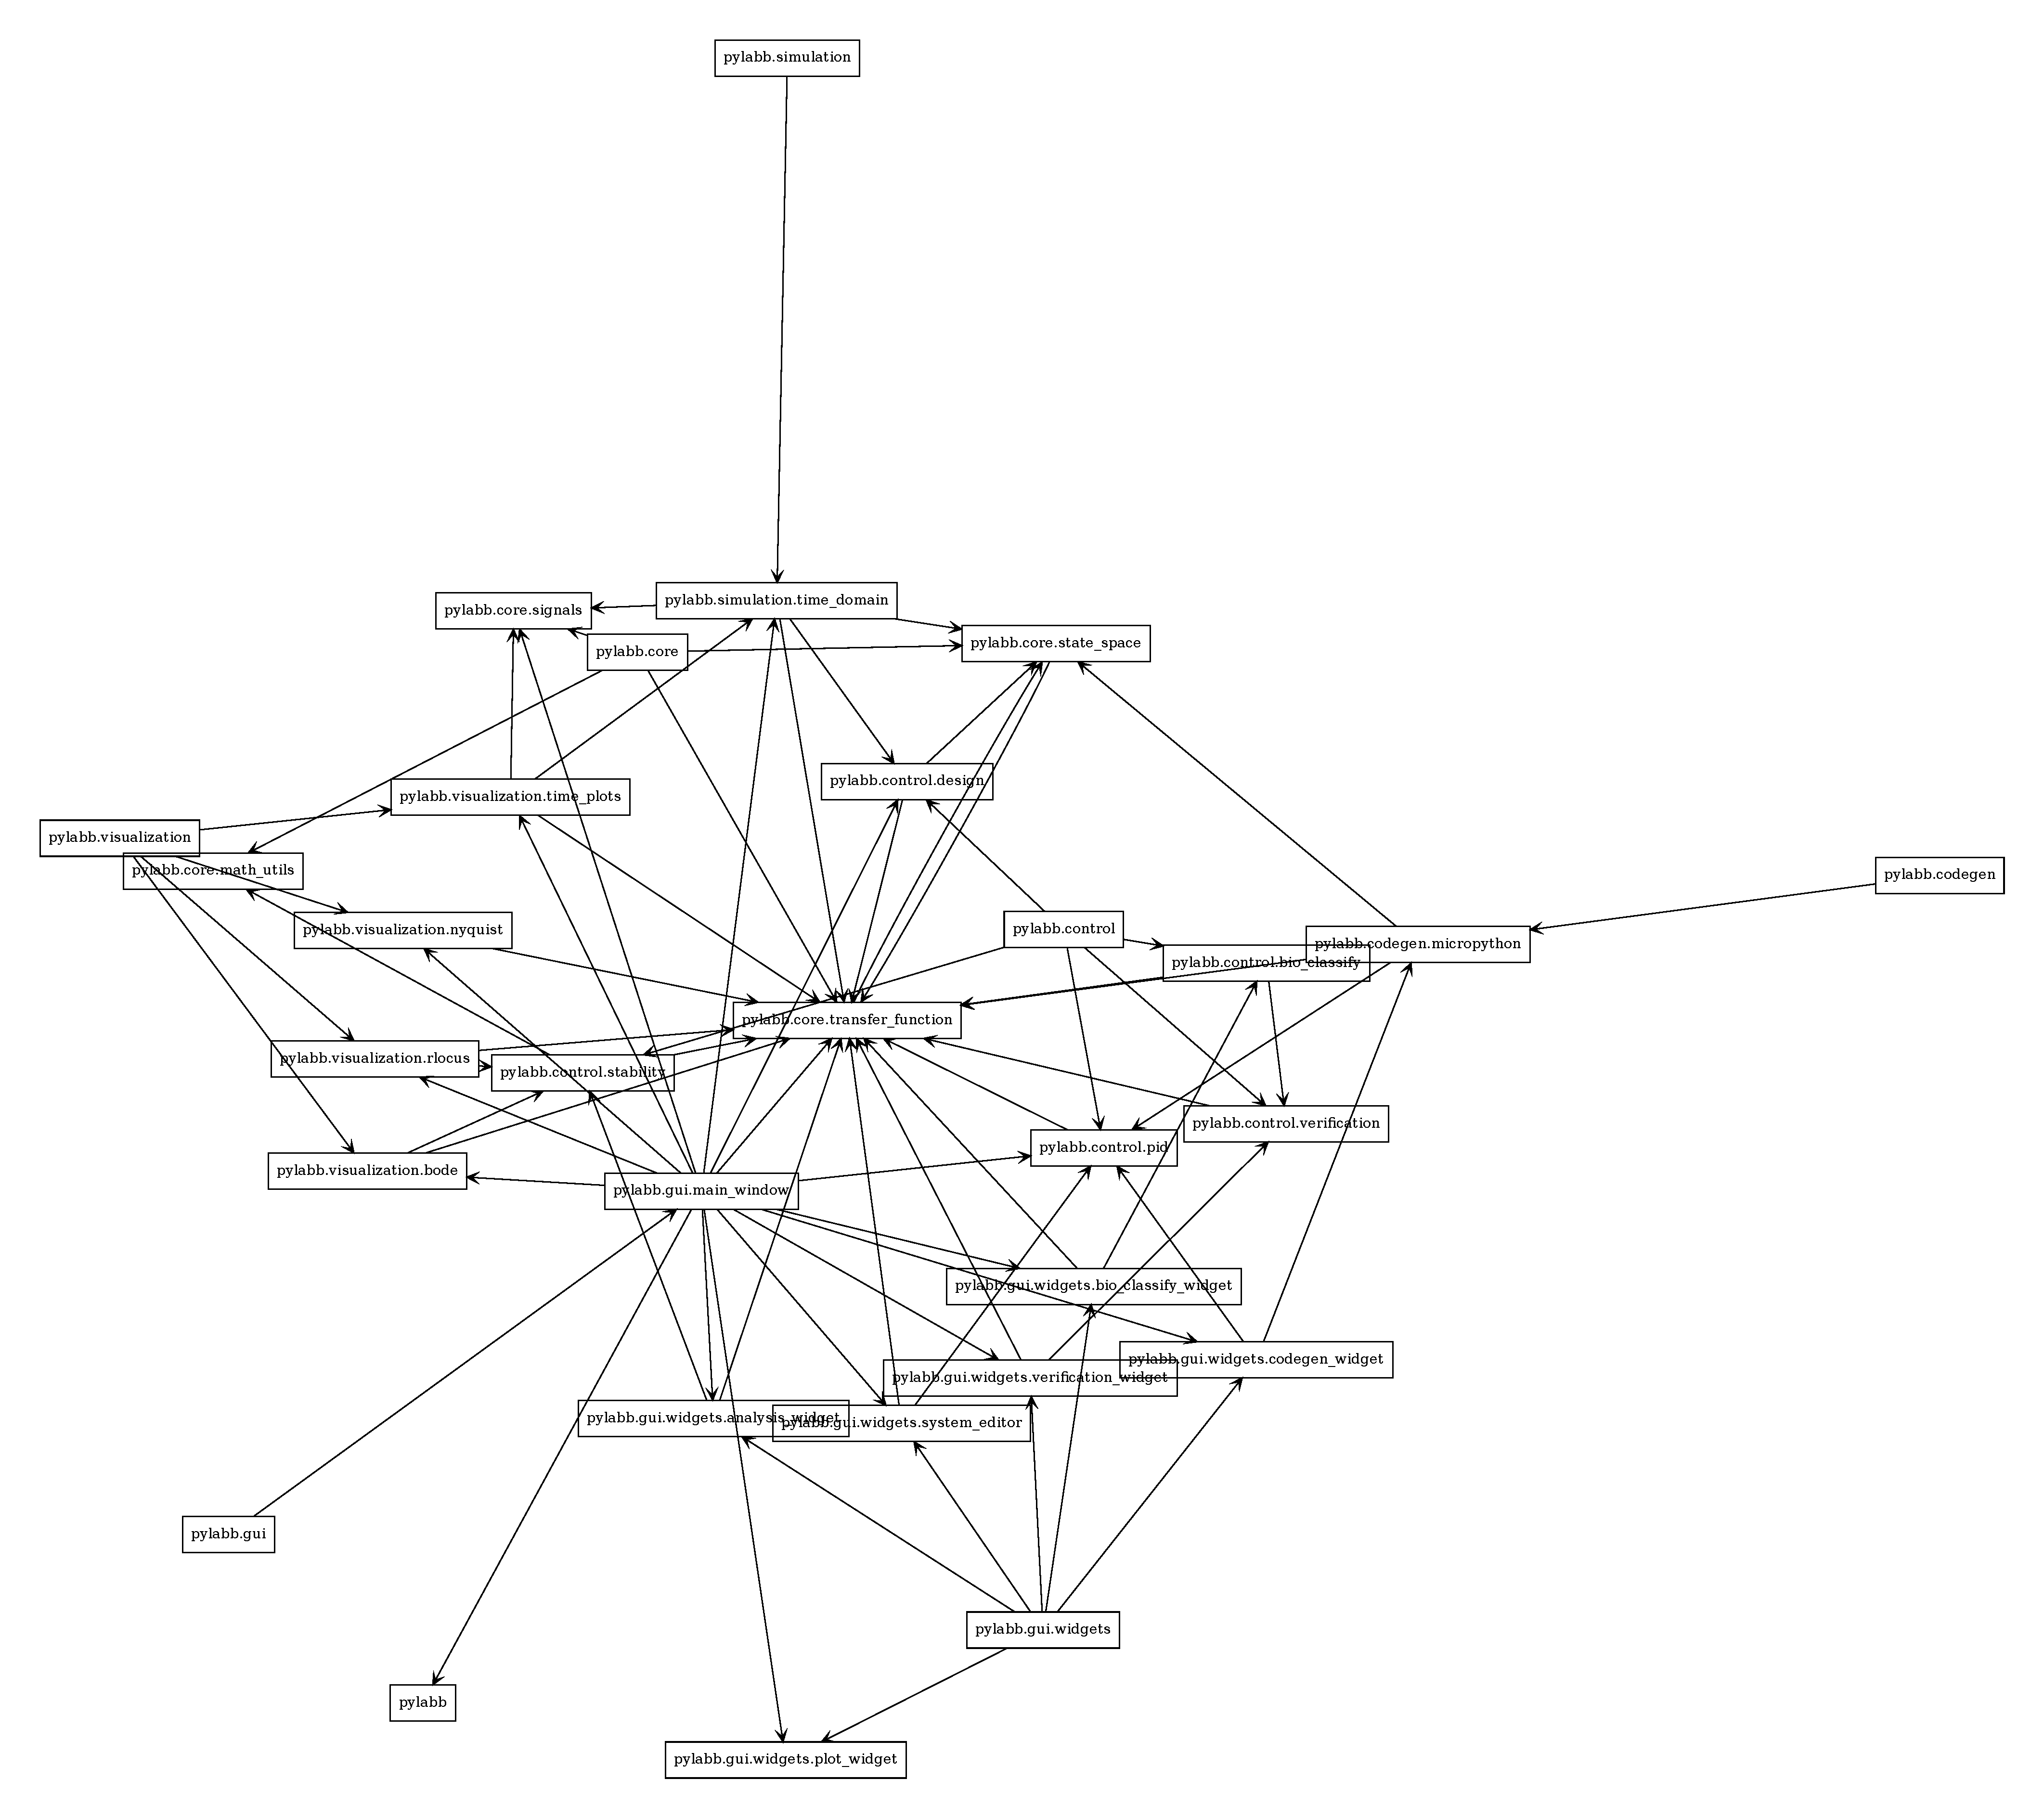
\includegraphics[width=0.75\linewidth]{../doc/uml/packages_pylabb.pdf}
    \caption{UML-Paketdiagramm von PyLab (generiert mit \texttt{pyreverse})}
    \label{fig:packages}
\end{figure}
\end{landscape}

\begin{landscape}
\begin{figure}[p]
    \centering
    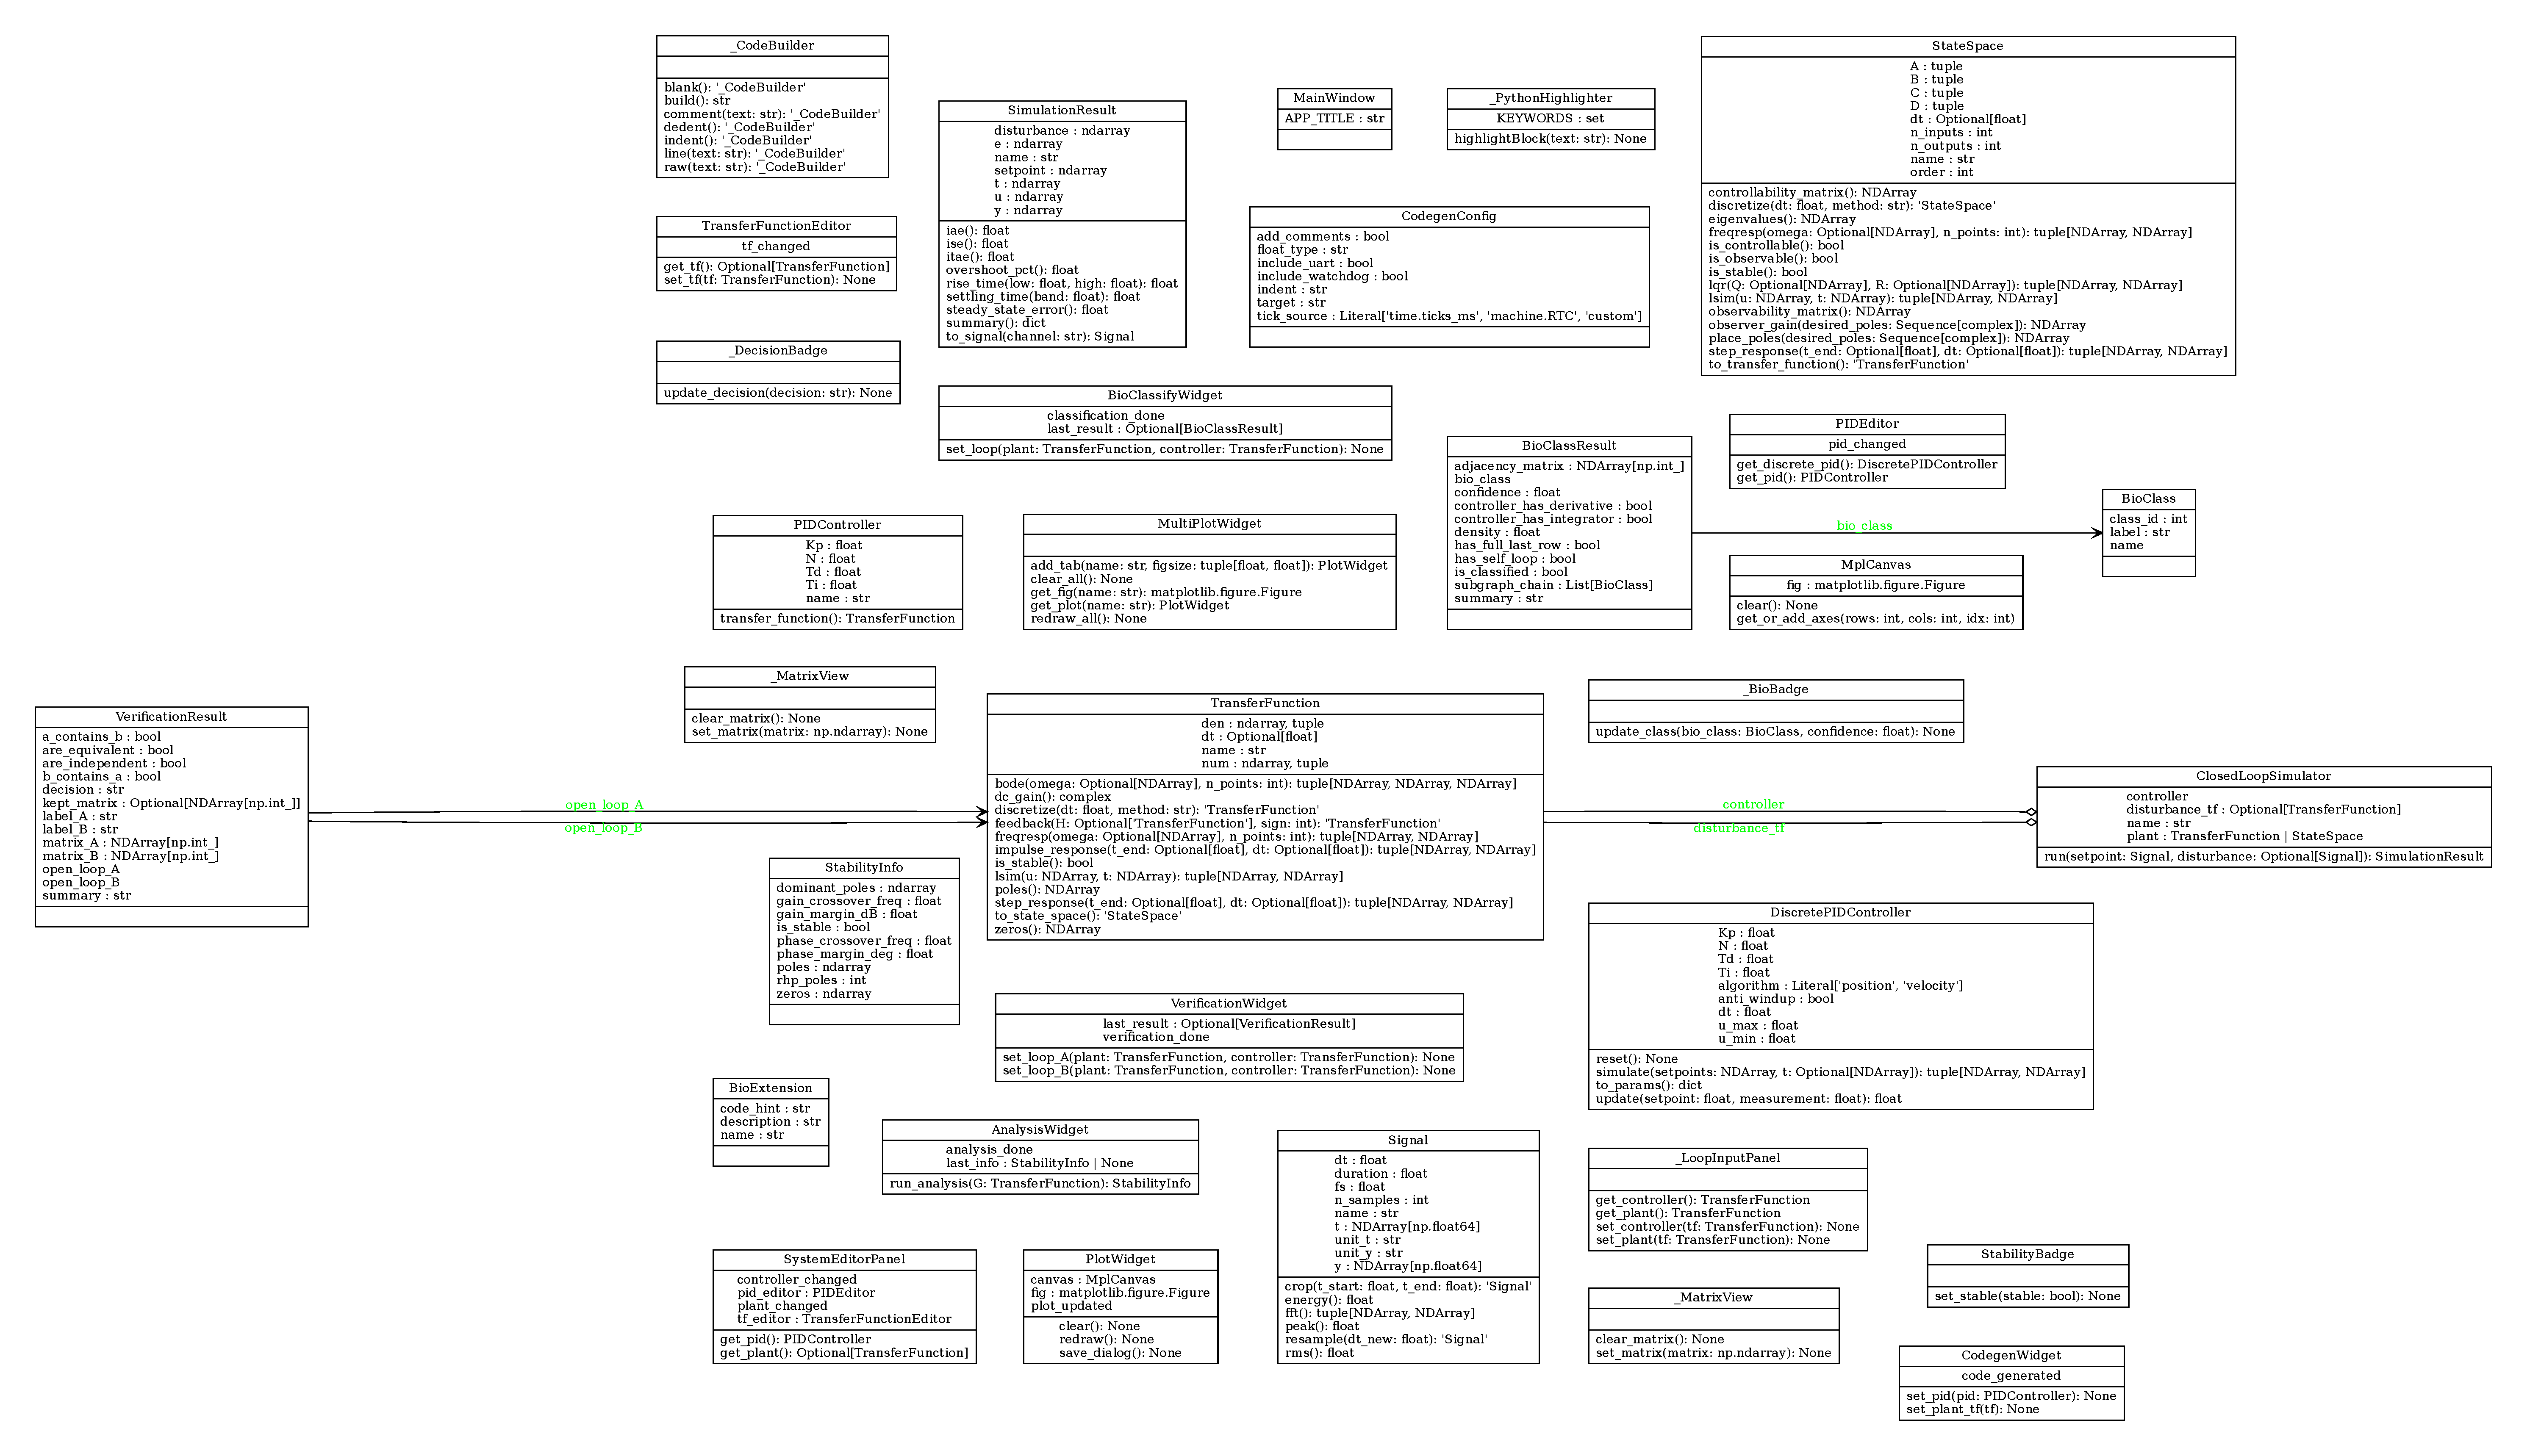
\includegraphics[width=1.1\linewidth]{../doc/uml/classes_pylabb.pdf}
    \caption{UML-Klassendiagramm von PyLab (generiert mit \texttt{pyreverse})}
    \label{fig:classes}
\end{figure}
\end{landscape}

\subsection{Kernklassen}

\subsubsection{\texttt{TransferFunction}}

Die Klasse \texttt{TransferFunction} kapselt eine rationale Übertragungsfunktion
durch Zähler- und Nennerkoeffizienten. Sie unterstützt algebraische Operatoren
(\texttt{+}, \texttt{*}, \texttt{/}), Pol-Nullstellen-Berechnung, Bode-Werte,
Impuls- und Sprungantwort sowie die Diskretisierung per Tustin- oder ZOH-Methode.

\subsubsection{\texttt{StateSpace}}

\texttt{StateSpace} repräsentiert ein System in der Form
$(\mathbf{A}, \mathbf{B}, \mathbf{C}, D)$ und bietet Methoden zur
Eigenwertberechnung, zur Simulation und zur Konvertierung in eine
Übertragungsfunktion.

\subsubsection{\texttt{PIDController} / \texttt{DiscretePIDController}}

Beide Klassen implementieren kontinuierliche bzw.\ diskrete PID-Regelgesetze
und generieren die zugehörige Übertragungsfunktion. Enthaltene Einstellregeln
sind Ziegler-Nichols~\cite{ziegler1942} (Sprung- und Schwingungsversuch),
Cohen-Coon~\cite{cohencoon} und $\lambda$-Tuning~\cite{astrom}.

% ============================================================
\section{Regelkreis-Verifikation}
\label{sec:verifikation}
% ============================================================

Die Verifikation von Regelkreisen ist das zentrale Thema dieser Arbeit.
Das Modul \texttt{pylabb.control.verification} implementiert ein
graphenstrukturelles Äquivalenzprü\-fungs\-verfahren, das auf dem
Subgraph Algorithmus~\cite{subgraph} basiert.

\subsection{Grundidee}

Zwei Regelkreise gelten als \emph{graphenstrukturell äquivalent}, wenn
ihre Signalflussgraphen isomorph sind oder einer den anderen als Subgraph
enthält. Die Parameterwerte der Übertragungsfunktionen spielen dabei keine
Rolle -- es wird ausschließlich die Topologie der Zustandskopplungsstruktur
verglichen.

\textbf{Anwendungsszenarien:}
\begin{itemize}
    \item Prüfung, ob ein einfacherer Regelkreis (z.\,B.\ P-Regler) in einem
          komplexeren (z.\,B.\ PID-Regler) strukturell enthalten ist.
    \item Nachweis der Gleichwertigkeit zweier Entwurfsalternativen
          hinsichtlich ihrer inneren Dynamik.
    \item Automatisierte Reduktion redundanter Regelkreisentwürfe in
          Entwurfsdatenbanken.
\end{itemize}

\subsection{Verarbeitungspipeline}

Die Verifikation läuft in vier Schritten ab:

\begin{enumerate}
    \item \textbf{Offenen Kreis berechnen:} $L_A(s) = C_A(s) \cdot G_A(s)$
          und $L_B(s) = C_B(s) \cdot G_B(s)$ durch Polynommultiplikation
          von Zähler und Nenner.

    \item \textbf{Zustandsraumdarstellung:} Scipy's \texttt{tf2ss}~\cite{scipy} überführt
          $L(s)$ in die Observable Canonical Form~\cite{ogata} und liefert die
          Systemmatrix~$\mathbf{A}$.

    \item \textbf{Adjazenzmatrix erzeugen:} Einträge $|\mathbf{A}_{ij}| > \varepsilon$
          werden auf 1 gesetzt, alle anderen auf 0.

    \item \textbf{Subgraph Algorithmus:} Die beiden Adjazenzmatrizen werden
          dem Algorithmus übergeben, der die Entscheidung zurückgibt.
\end{enumerate}

\begin{figure}[h]
\centering
\small
\[
\boxed{G_A(s),\,C_A(s)}
\;\rightarrow\;
\boxed{L_A(s) = C_A \cdot G_A}
\;\rightarrow\;
\boxed{\mathbf{A}_A}
\;\rightarrow\;
\boxed{\mathbf{M}_A \in \{0,1\}^{n \times n}}
\;\rightarrow\;
\text{\textbf{Subgraph Algo.}}
\]
\caption{Verarbeitungspipeline der Regelkreis-Verifikation (für Regelkreis A)}
\label{fig:pipeline}
\end{figure}

\subsection{Der Subgraph Algorithmus}

Der Subgraph Algorithmus~\cite{subgraph} prüft, ob ein Graph $G$ in einem
anderen Graphen $G'$ enthalten ist, ohne alle $n!$ Permutationen zu
enumerie\-ren. Stattdessen werden nur $n$ zyklische Rotationen der
Adjazenzmatrix betrachtet.

\subsubsection{Signaturen}

Für jede Spalte $j$ der Adjazenzmatrix wird eine eindeutige Signatur berechnet:
\[
\sigma_j = \sum_{i=0}^{n-1} A_{ij} \cdot 2^i + j \cdot 2^n \,.
\]

\begin{lemma}[Eindeutigkeit der Signaturen]
Die Signaturabbildung $\sigma: \{0,1\}^n \times \{0,\ldots,n-1\} \to \mathbb{N}$
ist injektiv.
\end{lemma}

\begin{proof}
Der Term $\sum_{i} A_{ij} \cdot 2^i$ interpretiert den Spaltenvektor als
Binärzahl und ist daher für unterschiedliche Muster verschieden. Der
Offset $j \cdot 2^n$ verschiebt gleiche Muster an verschiedenen Spalten
in disjunkte Wertebereiche $[j \cdot 2^n,\,(j+1)\cdot 2^n)$.
\end{proof}

\subsubsection{Zyklische Rotation}

Statt alle $n!$ Knotenpermutationen zu prüfen, rotiert der Algorithmus die
Spaltenreihenfolge der Adjazenzmatrix zyklisch. Dies erhält die sequentielle
Ordnung des Graphen und reduziert die Suchtiefe von $O(n!)$ auf $O(n)$.

\begin{beispiel}
Für $n = 4$ Spalten ergeben sich exakt vier Rotationen statt $4! = 24$
Permutationen:
\begin{align*}
\text{Rotation 0:} & \quad [\sigma_0, \sigma_1, \sigma_2, \sigma_3] \\
\text{Rotation 1:} & \quad [\sigma_1, \sigma_2, \sigma_3, \sigma_0] \\
\text{Rotation 2:} & \quad [\sigma_2, \sigma_3, \sigma_0, \sigma_1] \\
\text{Rotation 3:} & \quad [\sigma_3, \sigma_0, \sigma_1, \sigma_2]
\end{align*}
\end{beispiel}

\subsubsection{Subgraph-Kriterium}

\begin{satz}[Subgraph-Kriterium]
Eine Subgraph-Beziehung $G \subseteq G'$ wird genau dann erkannt, wenn
die längste gemeinsame Teilsequenz (LCS)~\cite{cormen} der Signatur-Arrays mindestens
die Länge~2 hat.
\end{satz}

\begin{proof}
Eine Subgraph-Beziehung erfordert mindestens eine Kante, d.\,h.\ mindestens
zwei Knoten mit Verbindung. Dies entspricht einer gemeinsamen Teilsequenz der
Signatur-Arrays der Länge $\geq 2$.
\end{proof}

\subsection{Entscheidungen des Algorithmus}

\begin{table}[h]
\centering
\begin{tabular}{@{}ll p{7cm}@{}}
\toprule
\textbf{Entscheidung} & \textbf{Python-Wert} & \textbf{Bedeutung} \\
\midrule
Äquivalent              & \texttt{"equal"}        & Beide Graphen sind strukturell identisch \\
Äquivalent (A bevorzugt)& \texttt{"equal\_keep\_A"}& Äquivalent; $G_A$ hat $\geq$ so viele Kanten wie $G_B$ \\
Äquivalent (B bevorzugt)& \texttt{"equal\_keep\_B"}& Äquivalent; $G_B$ hat mehr Kanten \\
A enthält B             & \texttt{"keep\_A"}       & $G_B \subseteq G_A$; Regelkreis A ist komplexer \\
B enthält A             & \texttt{"keep\_B"}       & $G_A \subseteq G_B$; Regelkreis B ist komplexer \\
Unabhängig              & \texttt{"keep\_both"}    & Keine strukturelle Inklusion; beide behalten \\
\bottomrule
\end{tabular}
\caption{Entscheidungen des Subgraph Algorithmus in der Regelkreis-Verifikation}
\label{tab:decisions}
\end{table}

\subsection{Implementierung: \texttt{verification.py}}

Das Modul \texttt{pylabb/control/verification.py} stellt drei öffentliche
Bezeichner bereit:

\begin{lstlisting}[language=Python, caption=Öffentliche API des Verifikationsmoduls]
from pylabb.control.verification import (
    loop_to_graph,        # Regelkreis -> (Adjazenzmatrix, L(s))
    verify_loops,         # Zwei Regelkreise vergleichen
    VerificationResult,   # Datenklasse für das Ergebnis
)
\end{lstlisting}

Die Funktion \texttt{loop\_to\_graph} wandelt einen Regelkreis in seinen
Signalflussgraphen um:

\begin{lstlisting}[language=Python, caption=Implementierung von loop\_to\_graph]
def loop_to_graph(plant, controller, threshold=1e-9):
    L = _open_loop(plant, controller)      # L(s) = C(s) * G(s)
    A, _B, _C, _D = sp_sig.tf2ss(          # Observable Canonical Form
        L.num.real, L.den.real
    )
    adj = (np.abs(A) > threshold).astype(int)
    return adj, L
\end{lstlisting}

Die Hauptfunktion \texttt{verify\_loops} führt die vollständige Verifikation
durch:

\begin{lstlisting}[language=Python, caption=Implementierung von verify\_loops (gekürzt)]
def verify_loops(plant_A, controller_A, plant_B, controller_B, ...):
    from subgraph import Subgraph  # ImportError wenn nicht installiert

    adj_A, L_A = loop_to_graph(plant_A, controller_A)
    adj_B, L_B = loop_to_graph(plant_B, controller_B)

    # Matrizen auf gemeinsame Größe bringen (Zero-Padding)
    if adj_A.shape[0] != adj_B.shape[0]:
        n_max = max(adj_A.shape[0], adj_B.shape[0])
        # ... zero-padding auf n_max x n_max ...

    algo = Subgraph()
    decision, kept = algo.compare_graphs(mat_A.astype(float),
                                          mat_B.astype(float))
    return VerificationResult(decision=decision, ...)
\end{lstlisting}

\subsection{Datenklasse \texttt{VerificationResult}}

Das Ergebnisobjekt kapselt alle relevanten Informationen:

\begin{lstlisting}[language=Python, caption=VerificationResult-Klasse]
@dataclass
class VerificationResult:
    decision:     str                  # Algorithmus-Entscheidung
    matrix_A:     NDArray[np.int_]     # Adjazenzmatrix Regelkreis A
    matrix_B:     NDArray[np.int_]     # Adjazenzmatrix Regelkreis B
    kept_matrix:  Optional[NDArray]    # Bevorzugte Matrix (oder None)
    open_loop_A:  TransferFunction     # L_A(s)
    open_loop_B:  TransferFunction     # L_B(s)
    label_A:      str                  # Beschriftung A
    label_B:      str                  # Beschriftung B

    # Bequemlichkeits-Properties
    @property
    def are_equivalent(self) -> bool: ...
    @property
    def a_contains_b(self)  -> bool: ...
    @property
    def b_contains_a(self)  -> bool: ...
    @property
    def are_independent(self) -> bool: ...
    @property
    def summary(self) -> str: ...
\end{lstlisting}

\subsection{Padding unterschiedlich großer Graphen}

Haben die beiden offenen Kreise verschiedene Ordnungen $n_A \neq n_B$,
werden beide Adjazenzmatrizen auf die Größe $n_{\max} \times n_{\max}$
mit Nullen aufgefüllt:
\[
\mathbf{M}_A^{\mathrm{pad}} = \begin{pmatrix} \mathbf{M}_A & \mathbf{0} \\ \mathbf{0} & \mathbf{0} \end{pmatrix} \in \{0,1\}^{n_{\max} \times n_{\max}}
\]

Dies stellt sicher, dass der Subgraph Algorithmus stets auf gleich großen
Matrizen operiert, während die ursprüngliche Knotenanzahl im Ergebnisobjekt
erhalten bleibt.

% ============================================================
\section{Biologisch orientierte Äquivalenzklassen von Regelkreisen}
\label{sec:bio_aequivalenz}
% ============================================================

\subsection{Motivation und Erkenntnisziel}

Die Regelungstechnik ist eine abstrakte Disziplin: Übertragungsfunktionen,
Zustandsraumdarstellungen und Signalflussgraphen beschreiben das dynamische
Verhalten technischer Systeme in einer Sprache der Mathematik. Gleichzeitig hat
die Natur im Laufe von Millionen Jahren der Evolution hocheffiziente Regelkreise
entwickelt -- in Tieren, Organen und Zellen -- die technischen Systemen in ihrer
Leistungsfähigkeit, Robustheit und Adaptivität weit überlegen sind.

Das Ziel dieses Kapitels ist es, eine systematische Klassifikation von
technischen Regelkreisen \emph{nach biologischen Vorbildern} zu entwickeln.
Dabei wird folgende Kernthese verfolgt:

\begin{quote}
	\textit{Regelkreise, die graphenstrukturell äquivalent sind (im Sinne des
		Subgraph Algorithmus aus Kapitel~\ref{sec:verifikation}), können einer
		gemeinsamen biologischen Regelklasse zugeordnet werden. Diese Zuordnung
		eröffnet die Möglichkeit, aus dem Verhalten des biologischen Vorbildes
		erweiterte Funktionen und Entwurfsstrategien für den technischen Regelkreis
		abzuleiten.}
\end{quote}

Die Idee verbindet zwei Forschungsrichtungen:
\begin{itemize}
	\item die \textbf{Bionik der Regelungstechnik}, also die Übertragung
	biologischer Prinzipien auf technische Systeme~\cite{ogata,lunze}, und
	\item die \textbf{graphenstrukturelle Verifikation} aus
	Kapitel~\ref{sec:verifikation}, die eine formale Äquivalenz\-prüfung
	von Regelkreisen ermöglicht.
\end{itemize}

\paragraph{Warum biologische Vorbilder?}
Lebewesen sind evolutionär optimierte Regelungssysteme. Das menschliche Auge
kompensiert Beleuchtungsänderungen über sechs Dekaden, die Körpertemperatur
wird auf $\pm 0{,}5\,°C$ gehalten, das vestibuläre System balanciert einen
aufrecht gehenden Menschen gegen Störungen -- alles ohne explizit programmierten
Reglerentwurf. Diese biologischen Systeme verkörpern \emph{optimale Lösungen}
regelungstechnischer Probleme. Wer versteht, welcher abstrakte Regelkreistyp
einem biologischen Organ entspricht, kann aus dem biologischen Verhalten
qualitative und quantitative Entwurfshinweise für technische Systeme gewinnen.

\paragraph{Abgrenzung.}
Dieses Kapitel ist \emph{keine} Einführung in die Neurobiologie oder
Physiologie. Es betrachtet biologische Systeme ausschließlich aus der Perspektive
der Regelungstechnik: als Regelstrecken, Regler, Sollwertgeber und
Rückführzweige. Die biologischen Beschreibungen sind vereinfacht und dienen
dem Zweck der regelungstechnischen Analogiebildung.

% ============================================================
\subsection{Grundlegende Konzepte der biologischen Regelung}
\label{subsec:bio_grundlagen}
% ============================================================

\subsubsection{Hierarchische Regelkreisstruktur in Lebewesen}

Biologische Regelungssysteme sind grundsätzlich hierarchisch organisiert.
In einem Säugetier lassen sich mindestens vier Regelungsebenen unterscheiden:

\begin{table}[h]
	\centering
	\begin{tabular}{@{}clp{6.5cm}@{}}
		\toprule
		\textbf{Ebene} & \textbf{Biologisches System} & \textbf{Regelungstechnisches Äquivalent} \\
		\midrule
		4 & Kortikale Verhaltenssteuerung     & Hierarchischer Mehrgrößenregler (MIMO), Sollwertvorgabe \\
		3 & Hormonelles System                & Langsamer integrierender Regler mit großer Totzeit \\
		2 & Autonomes Nervensystem            & Schneller nichtlinearer Rückführregler \\
		1 & Zelluläre Homöostase              & Lokaler Proportionalregler mit Sättigung \\
		\bottomrule
	\end{tabular}
	\caption{Hierarchische Regelungsebenen in Säugetieren}
	\label{tab:bio_ebenen}
\end{table}

Jede dieser Ebenen weist charakteristische dynamische Eigenschaften auf:
unterschiedliche Zeitkonstanten (Millisekunden bis Tage), unterschiedliche
Reglerstrukturen (P, PI, PID, nichtlinear) und unterschiedliche
Signaltypen (elektrische Impulse, chemische Gradienten, mechanische Kraft).

\subsubsection{Gemeinsame Eigenschaften biologischer Regelkreise}

Biologische Regelkreise teilen eine Reihe von Eigenschaften, die für die
Klassifikation relevant sind:

\begin{description}
	\item[Robustheit gegenüber Parameterunsicherheit.]
	Biologische Systeme funktionieren trotz erheblicher Variabilität in
	Parametern (Körpermasse, Körpertemperatur, Alter). Dies entspricht
	dem Entwurfsziel \emph{robuste Regelung} in der Regelungstechnik.
	
	\item[Adaptivität.]
	Biologische Regler passen ihre Parameter an veränderte Bedingungen an
	(Lernen, Akklimatisation). Dies entspricht \emph{adaptiver Regelung}
	oder \emph{selbsteinstellenden Reglern}.
	
	\item[Vorsteuersignal (Feedforward).]
	Viele biologische Systeme reagieren nicht nur rückge\-koppelt, sondern
	antizipieren Störungen. Das Kleinhirn beispielsweise berechnet
	motorische Korrekturen \emph{vor} der Ausführung einer Bewegung.
	Dies entspricht einer \emph{Vorsteuerung} oder \emph{Smith-Prädiktor}-
	Struktur in der technischen Regelungstechnik.
	
	\item[Mehrfachrückkopplung.]
	Biologische Regelkreise besitzen fast immer mehrere Rückkopp\-lungspfade
	auf verschiedenen Zeitskalen. Dies entspricht \emph{kaskadiert
		verschalteten Regelkreisen}.
	
	\item[Nichtlinearität.]
	Sättigung, Schwellwerte (z.\,B.\ Aktionspotential) und Hysterese sind
	biologischen Systemen inhärent. Entsprechend enthält jede biologisch
	motivierte Regelklasse nichtlineare Erweiterungen des Grundtyps.
\end{description}

% ============================================================
\subsection{Definition der biologischen Äquivalenzklassen}
\label{subsec:bio_klassen_definition}
% ============================================================

\begin{definition}[Biologische Äquivalenzklasse]
	Zwei Regelkreise $\mathcal{L}_A = (C_A(s), G_A(s))$ und
	$\mathcal{L}_B = (C_B(s), G_B(s))$ gehören zur selben \emph{biologischen
		Äquivalenzklasse} $\mathcal{K}_\beta$, wenn:
	\begin{enumerate}
		\item ihre Signalflussgraphen graphenstrukturell äquivalent sind (gemäß
		Subgraph Algorithmus, Kapitel~\ref{sec:verifikation}),
		\item die charakteristischen Frequenzeigenschaften (Bandbreite, Phasenlage,
		Integralanteil) mit dem biologischen Vorbild $\beta$ übereinstimmen, und
		\item die qualitativen Stellgrößen- und Regelgrößenverläufe dem biologischen
		Regelverhalten entsprechen.
	\end{enumerate}
	Das biologische Vorbild $\beta$ ist das Tier, Organ oder Teilsystem, dessen
	Regelstruktur als Referenz dient.
\end{definition}

Im Folgenden werden sieben biologische Äquivalenzklassen ausführlich beschrieben.
Jede Klasse ist nach einem biologischen Vorbild benannt, das die wesentlichen
Eigenschaften des zugehörigen Regelkreistyps exemplarisch verkörpert.

% ============================================================
\subsection{Klasse I -- Der Seestern: Dezentrale Proportionalregelung}
\label{subsec:klasse_seestern}
% ============================================================

\subsubsection{Biologisches Vorbild: Seestern (\textit{Asteroidea})}

Der Seestern ist ein Stachelhäuter ohne zentrales Gehirn. Seine Fortbewegung
wird durch ein dezentrales Nervennetz gesteuert: Jeder der fünf Arme enthält
ein eigenes Ganglion, das die Tube-Feet (Saugnapffüße) des betreffenden Arms
autonom koordiniert. Eine zentrale Instanz, die alle Arme zusammenführt,
existiert nicht -- trotzdem bewegt sich der Seestern gerichtet und koordiniert.

\paragraph{Regelungstechnische Interpretation.}
Jeder Arm des Seesterns realisiert einen \emph{lokalen Proportionalregler}:
Der Stellreflex auf Berührung oder optische Gradienten erfolgt unmittelbar, ohne
zeitliche Integration. Die Koordination ergibt sich aus dem Kopplungsterm zwischen
den Armen: Wenn Arm 1 eine Bewegungsrichtung ``wählt'', werden die übrigen Arme
durch mechanische und neuronale Kopplung in dieselbe Richtung gezogen.

\begin{klasse}[Seestern -- Dezentrale Proportionalregelung]
	\label{kl:seestern}
	Die Seestern-Klasse umfasst alle Regelkreise mit folgenden Merkmalen:
	\begin{itemize}
		\item Rein proportionaler Regelanteil: Übertragungsfunktion des Reglers
		$C(s) = K_P$ (reelle Konstante).
		\item Kein Integralterm, kein bleibender Ausgleich.
		\item Signalflussgraph: Kettenstruktur oder vollständig verbundener Multigraph
		mit ausschließlich direkten Kanten (keine Rückkopplungsschleifen
		zweiter Ordnung).
		\item Adjazenzmatrix: dünn besetzt (wenige Kanten), reguläre Struktur
		(jeder Knoten hat denselben Eingrad und Ausgrad).
	\end{itemize}
\end{klasse}

\subsubsection{Graphenstruktur der Seestern-Klasse}

Die Systemmatrix $\mathbf{A}$ eines P-Reglers mit einer Strecke $n$-ter Ordnung
in Observable Canonical Form hat folgende Struktur:
\[
\mathbf{A}_{\text{Seestern}} =
\begin{pmatrix}
	0      & 1      & 0      & \cdots & 0      \\
	0      & 0      & 1      & \cdots & 0      \\
	\vdots &        & \ddots & \ddots & \vdots \\
	0      & 0      & \cdots & 0      & 1      \\
	-a_0   & -a_1   & \cdots & -a_{n-2} & -a_{n-1}
\end{pmatrix}
\]
Diese Matrix erzeugt einen \emph{gerichteten Pfadgraphen} $P_n$ mit einer
einzigen Rückführkante von $v_n$ nach $v_1, \ldots, v_n$. Die Adjazenzmatrix
$\mathbf{M}_{\text{Seestern}}$ ist eine obere Bidiagonale mit einer voll besetzten
letzten Zeile -- das charakteristische ``Seestern-Muster''.

\subsubsection{Abgeleitete Entwurfsstrategien}

Die biologische Analogie offenbart folgende Entwurfshinweise:

\begin{enumerate}
	\item \textbf{Verteilte Implementierung.} Wie beim Seestern können P-Regler
	für verteilte Systeme (z.\,B.\ mehrere ESP32-Knoten in einem Sensornetz)
	ohne zentrale Koordination implementiert werden. Jeder Knoten regelt
	seine lokale Größe; die Kopplung erfolgt durch gemeinsame physikalische
	Größen (Spannung, Druck) -- nicht durch explizite Kommunikation.
	\item \textbf{Fehlertoleranz.} Der Seestern überlebt den Verlust eines Arms.
	Entsprechend sollten P-Regler in sicherheitskritischen Systemen
	redundant ausgelegt werden: Fällt ein Regler-Knoten aus, übernehmen
	die verbleibenden die Regelung mit reduzierter Stellkraft.
	\item \textbf{Robuste Inbetriebnahme.} Ein P-Regler mit kleinem $K_P$ ist
	immer stabil (für stabile Strecken). Wie der Seestern ``ausprobiert'',
	in welche Richtung er sich bewegen soll, kann $K_P$ iterativ erhöht
	werden, bis die gewünschte Regeldynamik erreicht ist.
\end{enumerate}

\subsubsection{Erweiterungspotenzial aus der biologischen Analogie}

Die dezentrale Intelligenz des Seesterns legt nahe:

\begin{hypothese}[Seestern-Erweiterung]
	Ein Regelkreis der Seestern-Klasse kann durch Hinzufügen von
	\emph{Kommunikationspfaden} zwischen bisher isolierten P-Reglern zu einem
	\emph{konsens-basierten Mehrfachregler} erweitert werden. Die erweiterte
	Funktion ist die kollektive Optimierung eines gemeinsamen Gütekriterials ohne
	zentrale Instanz -- analog zu Ant-Colony-Optimierungsverfahren.
\end{hypothese}

% ============================================================
\subsection{Klasse II -- Pupille: Integrierender Regelkreis mit Sättigung}
\label{subsec:klasse_pupille}
% ============================================================

\subsubsection{Biologisches Vorbild: Pupillenreflex des Auges}

Der Pupillenreflex ist einer der am besten verstandenen Regelkreise in der
Biologie~\cite{astrom}. Er regelt den Lichteinfall auf die Netzhaut durch
Verstellung des Pupillendurchmessers. Die Regelgröße ist die Beleuchtungsstärke
auf der Netzhaut, die Stellgröße ist die Kontraktion des Musculus sphincter
pupillae (Verengung) oder des Musculus dilatator pupillae (Erweiterung).

\paragraph{Dynamisches Verhalten.}
Das Pupillensystem zeigt folgende charakteristische Merkmale:
\begin{itemize}
	\item \textbf{Totzeit:} ca.\ $0{,}18\,\text{s}$ (Latenz der Photorezeptoren
	und Nervenleitung).
	\item \textbf{Zeitkonstante:} ca.\ $0{,}1\,\text{s}$ (mechanische Reaktion
	des Muskels).
	\item \textbf{Sättigung:} Pupillendurchmesser begrenzt zwischen
	$1{,}5\,\text{mm}$ (maximale Kontraktion) und $8\,\text{mm}$
	(maximale Dilatation) -- ein Bereich von ca.\ 28\,dB Dämpfung.
	\item \textbf{Nichtlinearität:} Die Helligkeitswahrnehmung folgt dem
	Weber-Fechner-Gesetz (logarithmisch), was die effektive Verstärkung
	bei hohen Lichtintensitäten reduziert.
\end{itemize}

\begin{klasse}[Pupille -- PI-Regelung mit Totzeit und Sättigung]
	\label{kl:pupille}
	Die Pupillen-Klasse umfasst alle Regelkreise mit:
	\begin{itemize}
		\item PI-Regler: $C(s) = K_P\left(1 + \frac{1}{T_I s}\right)$, wobei der
		Integralterm den bleibenden Regelungsfehler eliminiert.
		\item Totzeitglied in der Strecke: $G(s) = G_0(s) \cdot e^{-T_t s}$
		mit $T_t > 0$.
		\item Stellgrößenbeschränkung (Sättigung): $|u(t)| \leq u_{\max}$.
		\item Signalflussgraph: Kettenstruktur mit zusätzlichem selbstrückführendem
		Knoten (der Integralzustand erzeugt eine Schleife $v_1 \to v_1$).
	\end{itemize}
\end{klasse}

\subsubsection{Graphenstruktur der Pupillen-Klasse}

Der Integralanteil eines PI-Reglers fügt einen Zustandsknoten $v_I$ hinzu,
der ausschließlich Selbstkopplung hat (Integralzustand $\dot{x}_I = e$,
$x_I \to x_I$). Die Adjazenzmatrix enthält daher einen Diagonaleintrag:
\[
\mathbf{M}_{\text{Pupille}} =
\begin{pmatrix}
	1      & 0      & 0      & \cdots \\
	1      & 0      & 1      & \cdots \\
	0      & 0      & 0      & \ddots \\
	\vdots & \vdots & \ddots & \ddots
\end{pmatrix}
\]
Die Selbstschleife bei $v_I$ (Eintrag $M_{11} = 1$) ist das graphische
Erkennungsmerkmal der Pupillen-Klasse und unterscheidet sie von der
Seestern-Klasse durch genau einen zusätzlichen Diagonaleintrag.

\subsubsection{Abgeleitete Entwurfsstrategien}

\begin{enumerate}
	\item \textbf{Anti-Windup als biologisches Prinzip.}
	Das Auge verhindert ``Integratorsättigung'' durch neuronale Anpassung:
	Bei maximaler Pupillenverengung wird das Integrationssignal nicht
	weiter aufgestapelt. Für technische PI-Regler in PyLab sollte
	daher stets ein Anti-Windup-Mechanismus implementiert werden,
	sobald eine Sättigungsgrenze erkennbar ist.
	
	\item \textbf{Totzeitkompensation nach Smith.}
	Die biologische Totzeit des Pupillenreflexes führt zu
	Oszillationen bei schnellen Lichtsprüngen (Hippus-Phänomen).
	Technische Systeme der Pupillen-Klasse mit signifikanter Totzeit
	sollten mit einem Smith-Prädiktor erweitert werden, der die Totzeit
	aus der Rückkopplungsschleife ``herausnimmt''.
	
	\item \textbf{Logarithmische Skalierung der Eingangsgröße.}
	Das Weber-Fechner-Gesetz legt nahe, dass Regelstrecken mit sehr
	großem Dynamikbereich (mehr als 40\,dB) von einer logarithmischen
	Vorverarbeitung profitieren, da dies die effektive Streckenverstärkung
	über den gesamten Arbeitsbereich konstant hält.
\end{enumerate}

\subsubsection{Erweiterungspotenzial: Adaptiver PI-Regler}

\begin{hypothese}[Pupillen-Erweiterung]
	Die logarithmische Nichtlinearität des Pupillenreflexes liefert die
	Entwurfsregel: Für Regelstrecken mit mehr als 40\,dB Dynamikbereich soll
	die Reglerverstärkung $K_P$ als Funktion des aktuellen Betriebspunktes
	adaptiert werden:
	\[
	K_P(y) = \frac{K_{P,0}}{1 + \alpha \ln(1 + y/y_0)}
	\]
	wobei $\alpha$ den Grad der Nichtlinearität und $y_0$ den Nominalwert
	der Regelgröße beschreibt. Dies entspricht einer \emph{gainscheduled
		PI-Regelung}, motiviert durch das biologische Vorbild.
\end{hypothese}

% ============================================================
\subsection{Klasse III -- Das Kleinhirn: Vorsteuerung und Lernender Regler}
\label{subsec:klasse_kleinhirn}
% ============================================================

\subsubsection{Biologisches Vorbild: Kleinhirn (\textit{Cerebellum})}

Das Kleinhirn ist das Koordinationszentrum für motorische Funktionen beim
Menschen und bei Wirbeltieren. Es enthält etwa 50--80\,\% aller Neuronen des
menschlichen Gehirns und ist für die Feinabstimmung von Bewegungen
verantwortlich. Das Kleinhirn arbeitet als \emph{internes Modell} des
Bewegungsapparates: Es lernt im Laufe der Entwicklung, Korrekturbefehle
\emph{vor} der eigentlichen Bewegungsausführung zu berechnen.

\paragraph{Regelungstechnische Charakteristika.}
\begin{itemize}
	\item \textbf{Vorsteuerung (Feedforward):} Das Kleinhirn berechnet die
	erforderliche Muskelspannung \emph{auf Basis des Sollwertes}, nicht
	auf Basis des gemessenen Fehlers. Dies ist eine klassische
	Vorsteuerstruktur.
	\item \textbf{Lernmechanismus:} Durch Purkinje-Zellen und Kletterfasern
	wird das interne Modell iterativ verbessert -- ein biologisches
	Äquivalent zu iterativen Lernregelungen (\emph{Iterative Learning
		Control, ILC}).
	\item \textbf{Zeitkonstanten:} Motorische Korrekturen geschehen in
	50--100\,ms; die Lernphase (Motorisches Gedächtnis) über Wochen bis Jahre.
	\item \textbf{Störungsbeobachter:} Das Kleinhirn schätzt externe Störungen
	(Gewicht eines Objektes, Wind) anhand von Erwartungsmodellen.
\end{itemize}

\begin{klasse}[Kleinhirn -- PID mit Vorsteuerung und iterativem Lernen]
	\label{kl:kleinhirn}
	Die Kleinhirn-Klasse umfasst alle Regelkreise mit:
	\begin{itemize}
		\item PID-Rückführregler: $C(s) = K_P + \frac{K_I}{s} + K_D s$.
		\item Additiver Vorsteuerung $U_{\mathrm{FF}}(s) = F(s) \cdot W(s)$,
		wobei $F(s)$ das Vorsteuermodell und $W(s)$ den Sollwert bezeichnet.
		\item Einer Lernkomponente $\Delta U_k = L \cdot e_{k-1}$ (iterative
		Korrektur über Wiederholungszyklen $k$).
		\item Signalflussgraph: Komplexer Graph mit parallelen Pfaden (Rückkopplung
		und Vorwärtspfad) sowie einem separaten Speicherknoten für den
		Lernterm.
	\end{itemize}
\end{klasse}

\subsubsection{Graphenstruktur der Kleinhirn-Klasse}

Die Kleinhirn-Klasse zeichnet sich durch einen Signalflussgraphen mit
\emph{zwei parallelen Hauptpfaden} aus: einem Rückkopplungspfad (PID) und
einem Vorwärtspfad (Vorsteuerung). Die Adjazenzmatrix hat dementsprechend
Block-Struktur:
\[
\mathbf{M}_{\text{Kleinhirn}} =
\begin{pmatrix}
	\mathbf{M}_{\text{PID}} & \mathbf{0} \\
	\mathbf{C}_{\text{FF}}  & \mathbf{M}_{\text{FF}}
\end{pmatrix}
\]
wobei $\mathbf{M}_{\text{PID}}$ die Adjazenzmatrix des PID-Kreises,
$\mathbf{M}_{\text{FF}}$ die des Vorsteuermodells und
$\mathbf{C}_{\text{FF}}$ die Kopplung zwischen beiden darstellt.
Der Subgraph Algorithmus erkennt $\mathbf{M}_{\text{PID}}$ als Subgraph
von $\mathbf{M}_{\text{Kleinhirn}}$: Ein PID-Kreis ist in jedem Kleinhirn-
Kreis enthalten.

\subsubsection{Abgeleitete Entwurfsstrategien}

\begin{enumerate}
	\item \textbf{Iterative Learning Control (ILC).}
	Das Kleinhirn lernt aus jedem Bewegungszyklus. In technischen
	Anwendungen mit \emph{repetitiven Prozessen} (Roboterschweißen,
	Druckmaschinen, Windturbinen) sollte jeder Zyklus $k$ dazu genutzt
	werden, den Vorsteuerterm zu verbessern:
	\[
	u_{k+1}(t) = u_k(t) + \gamma \cdot e_k(t)
	\]
	mit Lernrate $\gamma \in (0, 1)$. PyLab kann einen solchen Lernterm
	als separaten Signalpfad im Signalflussgraphen abbilden.
	
	\item \textbf{Modellbasierte Vorsteuerung.}
	Ist ein Streckenmodell $\hat{G}(s)$ bekannt, lautet das optimale
	Vorsteuerglied $F(s) = \hat{G}^{-1}(s)$ (Streckeninverse). In der
	Praxis wird $F(s)$ auf einen kausalen, properen Anteil beschränkt.
	PyLab kann prüfen, ob die Vorsteuerstruktur zur Kleinhirn-Klasse
	gehört, indem es den erweiterten Graphen mit der
	Referenztopologie vergleicht.
	
	\item \textbf{Schätzung von Störmomenten.}
	Das Kleinhirn schätzt Trägheitskräfte, die bei der Bewegung auftreten.
	Analog sollte in robotischen Anwendungen ein
	\emph{Störgrößenbeobach\-ter} (Disturbance Observer) dem PID-Regler
	überlagert werden.
\end{enumerate}

\subsubsection{Erweiterungspotenzial: Biologisch motiviertes ILC-Modul}

\begin{hypothese}[Kleinhirn-Erweiterung]
	Für Regelkreise der Kleinhirn-Klasse, die in PyLab identifiziert werden,
	soll automatisch ein ILC-Modul (\texttt{pylabb.control.ilc}) generiert werden,
	das:
	\begin{itemize}
		\item den Vorsteuerterm $u_{\mathrm{FF},k}$ über Wiederholungszyklen lernt,
		\item die Konvergenz des Lernfehlers $\|e_k\|_2 \to 0$ überprüft, und
		\item MicroPython-Code für die Lernkomponente auf einem ESP32 generiert.
	\end{itemize}
	Dies ist eine direkte Erweiterung des \texttt{genmicropy}-Codegenerators
	(Kapitel~\ref{sec:architektur}) um biologisch motivierte Lernalgorithmen.
\end{hypothese}

% ============================================================
\subsection{Klasse IV -- Das Herz: Autonomer Taktgeber und Kaskadenregelung}
\label{subsec:klasse_herz}
% ============================================================

\subsubsection{Biologisches Vorbild: Herzkreislaufsystem}

Das menschliche Herz-Kreislauf-System ist ein Musterbeispiel für
\emph{Kaskadenregelung} mit autonomem Taktgeber. Der Sinusknoten generiert
ohne äußere Einwirkung Aktionspotenziale mit einer Grundfrequenz von
60--100\,min$^{-1}$. Das autonome Nervensystem (Sympathikus/Parasympathikus)
überlagert diesen Taktgeber mit einem Korrektursignal, das die Herzrate
an den Bedarf (körperliche Aktivität, Stress) anpasst.

\paragraph{Kaskadenstruktur.}
\begin{itemize}
	\item \textbf{Äußerer Regelkreis (langsam):} Sauerstoffversorgung des
	Gewebes als Regelgröße; Regelgröße ist der mittlere arterielle Druck
	(MAP). Zeitkonstante: 20--60\,s.
	\item \textbf{Innerer Regelkreis (schnell):} Herzrate als Stellgröße für
	den Druck; Herzrate wird durch den Sinusknoten direkt eingestellt.
	Zeitkonstante: 1--5\,s.
	\item \textbf{Barorezeptor-Reflex:} Drucksensoren in der Aortenbogenregion
	messen den Blutdruck direkt und schicken ein Korrektursignal an den
	Sinusknoten -- ein hochdynamischer lokaler Regelkreis mit Zeitkonstante
	$< 1\,\text{s}$.
\end{itemize}

\begin{klasse}[Herz -- Kaskadenregelung mit autonomem Taktgeber]
	\label{kl:herz}
	Die Herz-Klasse umfasst alle Regelkreise mit:
	\begin{itemize}
		\item Kaskadenstruktur: Ein äußerer PI-Regler $C_{\text{aussen}}(s)$ gibt
		den Sollwert für einen inneren P-Regler $C_{\text{innen}}(s)$ vor.
		\item Innerer Regelkreis mit deutlich größerer Bandbreite als äußerer.
		Als Faustregel gilt: $\omega_{\text{innen}} \geq 5\, \omega_{\text{aussen}}$.
		\item Einem autonomen Taktgeber (Oszillatorterm) im Signalflussgraphen.
		\item Signalflussgraph: Zwei verschachtelte Schleifen (innere und äußere
		Rückkopplung) mit einem zusätzlichen Oszillatorknoten.
	\end{itemize}
\end{klasse}

\subsubsection{Graphenstruktur der Herz-Klasse}

Die Kaskadenstruktur erzeugt einen Signalflussgraphen mit \emph{zwei
	konzentrischen Schleifen}. Die Adjazenzmatrix hat Block-Tridiagonalstruktur:
\[
\mathbf{M}_{\text{Herz}} =
\begin{pmatrix}
	\mathbf{M}_{\text{innen}} & \mathbf{K}_{ai} & \mathbf{0} \\
	\mathbf{0}                & \mathbf{M}_{\text{aussen}} & \mathbf{0} \\
	\mathbf{K}_{oi}           & \mathbf{0}                 & \mathbf{M}_{\text{osc}}
\end{pmatrix}
\]
wobei $\mathbf{K}_{ai}$ die Kopplung vom äußeren zum inneren Regler,
$\mathbf{K}_{oi}$ die Kopplung vom Oszillator zum inneren Kreis und
$\mathbf{M}_{\text{osc}} = \begin{pmatrix} 0 & 1 \\ -1 & 0 \end{pmatrix}$
die Adjazenzmatrix eines harmonischen Oszillators beschreibt.

\subsubsection{Abgeleitete Entwurfsstrategien}

\begin{enumerate}
	\item \textbf{Kaskadenregelung als Standardstruktur.}
	Der Herzkreislauf bestätigt das Entwurfsprinzip der Kaskadenregelung:
	Schnelle innere Störungen (Herzrhythmus) werden durch den inneren
	Kreis bereits kompensiert, bevor sie den äußeren Kreis beeinflussen.
	In technischen Systemen (z.\,B.\ Antriebsregelung: innerer
	Stromregelkreis, äußerer Drehzahlregelkreis) sollte dieselbe
	Hierarchie eingehalten werden.
	
	\item \textbf{Entwurf des inneren Kreises zuerst.}
	Das Herz entwirft den Sinusknoten evolutionär früher als die
	übergeordneten Regulierungsmechanismen. Analog ist in der technischen
	Kaskadenregelung stets der innere Regelkreis zuerst einzustellen
	(Ziegler-Nichols oder IMC~\cite{astrom}), bevor der äußere Regler
	parametriert wird.
	
	\item \textbf{Überwachung des Takt-Verhältnisses.}
	Der Sinusknoten wird überwacht (EKG). Analog sollte PyLab bei
	Kaskadenregelkreisen die Verhältnisse der Bandbreiten automatisch
	prüfen und eine Warnung ausgeben, wenn $\omega_{\text{innen}} <
	3\, \omega_{\text{aussen}}$ (drohende Instabilität des Kaskadensystems).
\end{enumerate}

\subsubsection{Erweiterungspotenzial: Pulsweitenmodulierter Antrieb}

\begin{hypothese}[Herz-Erweiterung]
	Das Herz moduliert die Herzrate (Frequenz) statt der Kontraktionsstärke
	(Amplitude). Dies entspricht Pulsweitenmodulation (PWM). Kaskadenregelkreise
	der Herz-Klasse, die auf Mikrocontrollern implementiert werden,
	sollten daher:
	\begin{itemize}
		\item den inneren Regelkreis als PWM-Regler mit variabler Frequenz
		implementieren,
		\item die Ausgangsperiode dynamisch an die Regelabweichung anpassen,
		\item und den äußeren PI-Regler mit deutlich kleinerer Abtastrate
		(mindestens Faktor 10) betreiben.
	\end{itemize}
	\texttt{genmicropy} soll diese Struktur als biologisch motivierten
	``Herz-Template'' automatisch generieren.
\end{hypothese}

% ============================================================
\subsection{Klasse V -- Der Albatros: Energieoptimale Regelung mit Windausnutzung}
\label{subsec:klasse_albatros}
% ============================================================

\subsubsection{Biologisches Vorbild: Albatros (\textit{Diomedea})}

Der Albatros ist der Meister der energieeffizienten Fortbewegung. Er verbringt
den größten Teil seines Lebens auf See und durchfliegt dabei Zehntausende von
Kilometern -- mit einem Energieverbrauch, der deutlich unter dem aller anderen
Vögel gleicher Größe liegt. Sein Geheimnis ist das \emph{dynamische
	Segeln}: Der Albatros nutzt den Windgradienten über der Meeresoberfläche
(schneller Wind oben, langsamerer Wind in Oberflächennähe) aus, indem er
kontrolliert zwischen diesen Schichten wechselt und dabei kinetische Energie
aus dem Wind ``erntet''.

\paragraph{Regelungstechnische Interpretation.}
Das dynamische Segeln ist eine \emph{zeitoptimale energieernternde Steuerung}.
Der Albatros maximiert $\int_{t_0}^{t_1} \mathbf{v}_{\text{wind}} \cdot \mathbf{v}_{\text{Albatros}}\,\mathrm{d}t$
unter der Nebenbedingung einer Mindestflughöhe. Dies entspricht einem
\emph{optimalen Regler} (LQR oder Pontryaginsches Maximumprinzip) mit einer
Nebenbedingung (Constraint).

\begin{klasse}[Albatros -- LQR mit Nebenbedingungen und Störgrößenauf\-schaltung]
	\label{kl:albatros}
	Die Albatros-Klasse umfasst alle Regelkreise mit:
	\begin{itemize}
		\item Zustandsrückkühlung durch einen optimal ausgelegten
		Rückführvektor: $C(s) \equiv \mathbf{k}^T$ (LQR-Regler).
		\item Störgrößenaufschaltung: Die messbare Störgröße $d(t)$ (Windgeschwindigkeit,
		externe Kraft) wird direkt in die Stellgröße eingerechnet.
		\item Beschränkter Stellgröße oder Zustand ($u_{\min} \leq u \leq u_{\max}$,
		$x_{\min} \leq x \leq x_{\max}$).
		\item Signalflussgraph: Vollständig verbundener Graph mit zusätzlichem
		Störeingangsknoten (Pendant zu den ``Wind''-Knoten des Albatros).
	\end{itemize}
\end{klasse}

\subsubsection{Graphenstruktur der Albatros-Klasse}

Ein LQR-Regler implementiert eine Zustandsrückkopplung $u = -\mathbf{k}^T \mathbf{x}$,
was im geschlossenen Kreis zu einer vollständig verbundenen letzten Zeile der
Systemmatrix führt. Die Adjazenzmatrix der Albatros-Klasse hat daher
\emph{mindestens eine vollständig besetzte Zeile} (die Rückführzeile):
\[
\mathbf{M}_{\text{Albatros}} =
\begin{pmatrix}
	0      & 1      & 0      & 0      \\
	0      & 0      & 1      & 0      \\
	0      & 0      & 0      & 1      \\
	1      & 1      & 1      & 1      \\
\end{pmatrix}
\quad \text{(Beispiel, } n=4\text{)}
\]
Hinzu kommt eine Spalte für den Störgrößenknoten $v_d$, der mit allen
Zustandsknoten verbunden ist (Albatros ``sieht'' den Wind an jedem Ort).

\subsubsection{Abgeleitete Entwurfsstrategien}

\begin{enumerate}
	\item \textbf{Messbare Störgrößen nutzen.}
	Der Albatros misst den Wind explizit (über Druckrezeptoren am
	Schnabel und den Stutzknochen der Flügelwurzel). In technischen
	Systemen sollten messbare Störgrößen (Netzfrequenz, Umgebungstemperatur,
	externe Kraft) stets direkt in den Regler aufgenommen werden --
	Störgrößenaufschaltung reduziert die erforderliche Regelverstärkung
	erheblich.
	
	\item \textbf{Energieoptimale Trajektorienplanung.}
	Das Segment-Segelverhalten des Albatros entspricht einer
	\emph{Model Predictive Control} (MPC): In jedem Zeitschritt wird
	über einen Horizont $H$ optimiert, welcher Flugpfad die maximale
	Energieausbeute liefert. PyLab könnte dies als MPC-Modul implementieren.
	
	\item \textbf{Ausbeutung periodischer Störungen.}
	Meereswellen (und damit der Windgradient) sind näherungsweise
	periodisch. Ein Resonanzfilter im Vorwärtspfad, der auf die
	dominante Wellenfrequenz abgestimmt ist, kann die
	Energieernte weiter steigern -- analoges biologisches Verhalten
	ist beim Albatros als ``Resonanzsegeln'' bekannt.
\end{enumerate}

\subsubsection{Erweiterungspotenzial: MPC-Modul für PyLab}

\begin{hypothese}[Albatros-Erweiterung]
	Regelkreise der Albatros-Klasse werden in PyLab automatisch als Kandidaten
	für eine MPC-Erweiterung identifiziert. Die Identifikation erfolgt durch:
	\begin{enumerate}
		\item Nachweis, dass die Adjazenzmatrix einen Störeingangsknoten enthält
		(Subgraph-Prüfung gegen eine Referenztopologie).
		\item Nachweis, dass die Rückführzeile vollständig besetzt ist (LQR-Struktur).
	\end{enumerate}
	Sind beide Bedingungen erfüllt, schlägt PyLab eine MPC-Parametrierung vor
	und berechnet den LQR-Verstärkungsvektor $\mathbf{k}$ über die
	Riccati-Gleichung.
\end{hypothese}

% ============================================================
\subsection{Klasse VI -- Die Mimose: Nichtlinearer Regelkreis mit Hysterese}
\label{subsec:klasse_mimose}
% ============================================================

\subsubsection{Biologisches Vorbild: Mimose (\textit{Mimosa pudica})}

Die Mimose ist eine Pflanze, die auf Berührungsreize mit dem blitzschnellen
Zusammenfalten ihrer Blätter reagiert (Seismonastie). Dieses Verhalten ist
eines der bekanntesten Beispiele für pflanzliche Reiz-Reaktions-Systeme.
Aus regelungstechnischer Sicht zeigt die Mimose folgende charakteristische
Eigenschaften:

\paragraph{Schwellwertverhalten (Trigger).}
Die Mimose reagiert erst ab einem \emph{Mindestierreiz} (Schwellwert). Kleine
Berührungen werden ignoriert -- ein klares Schwellwertverhalten, das dem
Schaltelement (Zweipunktregler, Schmitt-Trigger) entspricht.

\paragraph{Hysterese.}
Nach dem Zusammenfalten öffnen sich die Blätter erst nach einer Erholungszeit
von mehreren Minuten wieder. Dies ist eine ausgeprägte Hysterese: Der
Schließzustand wird erst verlassen, wenn eine deutlich längere Beruhigungszeit
vergangen ist als die initiale Reizzeit.

\paragraph{Ermüdung (Refractory Period).}
Wird die Mimose wiederholt stimuliert, wird die Reaktion schwächer und
schließlich bleibt sie aus -- eine Adaptation (Habituation), die dem
Anti-Windup-Mechanismus technischer Zweipunktregler ähnelt.

\begin{klasse}[Mimose -- Nichtlinearer Zweipunktregler mit Hysterese]
	\label{kl:mimose}
	Die Mimosen-Klasse umfasst alle Regelkreise mit:
	\begin{itemize}
		\item Zweipunktregler (Bang-Bang-Regler) mit Hysterese-Bandbreite $h$:
		\[
		u(t) = \begin{cases}
			+U_{\max} & \text{wenn } e(t) > +h/2 \\
			-U_{\max} & \text{wenn } e(t) < -h/2 \\
			u(t^-)    & \text{sonst (Hysterese)}
		\end{cases}
		\]
		\item Einem Ermüdungsterm: Nach $N$ Schaltzyklen wird $U_{\max}$ auf
		$U_{\max} \cdot \eta^N$ reduziert ($\eta < 1$).
		\item Signalflussgraph: Stark nichtlinearer Signalflussgraph mit
		einem Schaltknoten (diskontinuierliche Übertragungsfunktion).
		Die Adjazenzmatrix ist äquivalent zur Seestern-Klasse, jedoch
		mit einem markierten Schaltknoten.
	\end{itemize}
\end{klasse}

\subsubsection{Graphenstruktur der Mimosen-Klasse}

Der Zweipunktregler selbst hat keine rationale Übertragungsfunktion und
lässt sich daher nicht direkt über eine Zustandsraumdarstellung erfassen.
Stattdessen wird die \emph{lineare Näherung} (Äquivalente Linearisierung via
Describing Function) verwendet:
\[
C_{\text{eq}}(j\omega, a) = \frac{4 U_{\max}}{\pi a} \sqrt{1 - \left(\frac{h}{a}\right)^2}
- j\frac{4 U_{\max} h}{\pi a^2}
\]
Diese komplexwertige Verstärkung erzeugt eine Adjazenzmatrix, die strukturell
der Seestern-Klasse entspricht -- aber durch einen imaginären Anteil
(Phasenverschiebung durch Hysterese) ergänzt wird. PyLab identifiziert
Mimosen-Regelkreise durch:
\begin{enumerate}
	\item Strukturelle Äquivalenz zur Seestern-Klasse (P-Regler-Topologie), und
	\item Nachweis eines Hysterese-Parameters $h > 0$ in der Parametrierung.
\end{enumerate}

\subsubsection{Abgeleitete Entwurfsstrategien}

\begin{enumerate}
	\item \textbf{Optimale Hysteresebandbreite.}
	Die Mimose wählt ihre Hysteresebandbreite evolutionär optimal:
	klein genug, um auf echte Bedrohungen zu reagieren, groß genug,
	um Windböen zu ignorieren. Für technische Zweipunktregler
	(Thermostate, Druckregler) lautet die optimale Hysterese-Regel:
	$h \approx 2\,\sigma_n$, wobei $\sigma_n$ die Standardabweichung
	des Messrauschens ist.
	
	\item \textbf{Grenzzyklen als Designmerkmal.}
	Ein Zweipunktregler mit symmetrischer Strecke erzeugt immer einen
	Grenzzyklus (Daueroszillation). Die Amplitude und Frequenz des
	Grenzzyklus sind durch die Describing Function berechenbar.
	PyLab soll für Mimosen-Klassen-Regelkreise automatisch den
	resultierenden Grenzzyklus berechnen und anzeigen.
	
	\item \textbf{Habituation als Schutzmechanismus.}
	Der Ermüdungsterm der Mimose verhindert Stellgliedverschleiß durch
	Dauerschalten. Technisch entspricht dies einer \emph{minimalen
		Schaltfrequenzbegrenzung} (Dwell Time), die in sicherheitskritischen
	Anwendungen (Schaltschütze, Ventile) unbedingt implementiert werden
	sollte.
\end{enumerate}

% ============================================================
\subsection{Klasse VII -- Der Tintenfisch: Multivariable adaptive Regelung}
\label{subsec:klasse_tintenfisch}
% ============================================================

\subsubsection{Biologisches Vorbild: Tintenfisch (\textit{Octopus vulgaris})}

Der Tintenfisch ist eines der intelligentesten Wirbellosen und ein
außergewöhnliches Beispiel für dezentral-distribuierte Intelligenz kombiniert
mit adaptiver Umgebungsanpassung. Neun Zehntel seiner Neuronen befinden sich
in seinen acht Armen -- jeder Arm hat ein eigenes ``Gehirn'' und kann
autonom handeln, wird aber durch das zentrale Gehirn koordiniert.

\paragraph{Regelungstechnische Charakteristika.}
\begin{itemize}
	\item \textbf{Mehrgrößenregelung (MIMO):} Acht Arme, jeder mit hunderten
	von Saugnäpfen, werden als ein koordiniertes System gesteuert.
	Dies entspricht einem MIMO-System mit $n \gg 1$ Eingangs- und
	Ausgangsvariablen.
	\item \textbf{Farbanpassung:} Chromatophoren (Farbzellen) werden durch ein
	dezentrales Regelungsnetz gesteuert, das innerhalb von Millisekunden
	Farbmuster auf der Haut erzeugt. Jede Zelle ist ein lokaler
	Aktor mit eigenem Regelkreis; die Koordination erfolgt durch
	neuronale Muster.
	\item \textbf{Adaptive Steifigkeit der Arme:} Je nach Aufgabe (Greifen,
	Schwimmen, Abtasten) passen die Arme ihre mechanische Steifigkeit
	an. Dies entspricht \emph{impedanzgeregelten} Roboterarmen.
	\item \textbf{Lernen und Gedächtnis:} Tintenfische können Konditionierungsaufgaben
	lösen (klassische und operante Konditionierung), was auf einen
	adaptiven Lernmechanismus im zentralen Gangliensystem hindeutet.
\end{itemize}

\begin{klasse}[Tintenfisch -- Adaptive MIMO-Regelung mit verteilter Intelligenz]
	\label{kl:tintenfisch}
	Die Tintenfisch-Klasse umfasst alle Regelkreise mit:
	\begin{itemize}
		\item Mehrgrößenstruktur: $\mathbf{C}(s) \in \mathbb{R}^{m \times p}$,
		$\mathbf{G}(s) \in \mathbb{R}^{p \times m}$.
		\item Dezentrale lokale Regler auf Aktorebene und einem zentralen
		Koordinationsregler.
		\item Adaptiver Parameteranpassung: $K_{ij}(t) = K_{ij,0} + \Delta K_{ij}(t)$.
		\item Signalflussgraph: Vollständig verbundener Multigraph (jeder Zustand
		beeinflusst jeden anderen Zustand) -- die dichteste Klasse unter
		allen biologischen Äquivalenzklassen.
	\end{itemize}
\end{klasse}

\subsubsection{Graphenstruktur der Tintenfisch-Klasse}

Der Tintenfisch-Regelkreis erzeugt die dichteste Adjazenzmatrix aller
biologischen Klassen -- annähernd die vollständige Matrix:
\[
\mathbf{M}_{\text{Tintenfisch}} \approx \mathbf{J}_n = \begin{pmatrix} 1 & 1 & \cdots & 1 \\ 1 & 1 & \cdots & 1 \\ \vdots & & \ddots & \vdots \\ 1 & 1 & \cdots & 1 \end{pmatrix}
\]
Der Subgraph Algorithmus erkennt die Tintenfisch-Klasse daran, dass ihr
Signalflussgraph \emph{alle anderen biologischen Klassen als Subgraph enthält}:
$\mathbf{M}_{\text{Seestern}} \subseteq \mathbf{M}_{\text{Kleinhirn}} \subseteq
\mathbf{M}_{\text{Tintenfisch}}$ (vgl.\ Subgraph-Hierarchie
Kapitel~\ref{subsec:bio_hierarchie}).

\subsubsection{Abgeleitete Entwurfsstrategien}

\begin{enumerate}
	\item \textbf{Entkopplungsregler.}
	Ein vollständig verbundenes MIMO-System erfordert einen
	Entkopplungsregler, der die Quereinflüsse zwischen den Kanälen
	kompensiert. Die Tintenfisch-Klasse signalisiert daher in PyLab:
	``Entkopplung erforderlich!''
	
	\item \textbf{Impedanzregelung für Roboterarme.}
	Die adaptive Steifigkeit der Tintenfischarme ist das biologische
	Vorbild für impedanzgeregelte Manipulatoren. Die gewünschte
	Impedanz $Z_{\text{ref}}(s) = M s^2 + D s + K$ wird als Referenz-
	Übertragungsverhalten vorgegeben und der Regler so ausgelegt, dass
	er dieses Verhalten gegenüber äußeren Kräften durchsetzt.
	
	\item \textbf{Modellprädiktive MIMO-Regelung (MIMO-MPC).}
	Der Koordinationsmechanismus des zentralen Tintenfischgehirns
	entspricht einer modellprädiktiven Mehrgrößenregelung: Auf Basis
	eines internen MIMO-Modells werden optimale Eingaben für alle
	Kanäle gleichzeitig berechnet.
\end{enumerate}

\subsubsection{Erweiterungspotenzial: MIMO-Erweiterung von PyLab}

\begin{hypothese}[Tintenfisch-Erweiterung]
	Die Identifikation eines Regelkreises als Tinten\-fisch-Klasse motiviert die
	Erweiterung des Subgraph Algorithmus auf tensorproduktbasierte
	Graphen (vgl.\ Kapitel~\ref{sec:ausblick}). Die Tintenfisch-Klasse ist
	der natürliche Startpunkt für die MIMO-Erweiterung von PyLab:
	\begin{itemize}
		\item Erweiterung der \texttt{TransferFunction}-Klasse auf
		Übertragungsmatrizen.
		\item Erweiterung des Subgraph Algorithmus auf blockstrukturierte
		Adjazenzmatrizen.
		\item Automatische Synthese von Entkopplungsreglern bei erkannter
		Tintenfisch-Topologie.
	\end{itemize}
\end{hypothese}

% ============================================================
\subsection{Hierarchie der biologischen Äquivalenzklassen}
\label{subsec:bio_hierarchie}
% ============================================================

Die sieben biologischen Äquivalenzklassen bilden eine Hierarchie, die durch die
Subgraph-Relation geordnet ist. Eine Klasse $\mathcal{K}_\alpha$ ist
\emph{Unterklasse} von $\mathcal{K}_\beta$, wenn jeder Regelkreis in
$\mathcal{K}_\alpha$ graphenstrukturell in einem Regelkreis der Klasse
$\mathcal{K}_\beta$ enthalten ist:

\begin{satz}[Subgraph-Hierarchie der biologischen Klassen]
	\label{satz:bio_hierarchie}
	Für die biologischen Äquivalenz\-klassen gilt folgende Subgraph-Ordnung:
	\[
	\mathcal{K}_{\text{Seestern}} \subsetneq \mathcal{K}_{\text{Pupille}}
	\subsetneq \mathcal{K}_{\text{Kleinhirn}} \subsetneq \mathcal{K}_{\text{Herz}}
	\subsetneq \mathcal{K}_{\text{Albatros}} \subsetneq \mathcal{K}_{\text{Tintenfisch}}
	\]
	Die Mimosen-Klasse steht strukturell zwischen Seestern und Pupille, ist jedoch
	nicht mit den übrigen Klassen vergleichbar (nichtlinear):
	\[
	\mathcal{K}_{\text{Seestern}} \subsetneq \mathcal{K}_{\text{Mimose}} \not\subseteq \mathcal{K}_{\text{Pupille}}
	\]
\end{satz}

\begin{proof}[Beweisskizze]
	\begin{itemize}
		\item \textbf{Seestern $\subsetneq$ Pupille:} Der Integralknoten der
		Pupillen-Klasse (Selbstschleife $M_{11}=1$) ist nicht in der
		Seestern-Adjazenzmatrix enthalten. Jede Seestern-Adjazenzmatrix
		ist jedoch (nach Padding) ein Subgraph der Pupillen-Matrix.
		\item \textbf{Pupille $\subsetneq$ Kleinhirn:} Der Vorsteuerblock der
		Kleinhirn-Klasse fügt zusätzliche Knoten hinzu, enthält aber
		die vollständige Pupillen-Topologie als Subgraph.
		\item \textbf{Kleinhirn $\subsetneq$ Herz:} Der Kaskadenblock der Herz-Klasse
		enthält zwei verschachtelte Schleifen; die Kleinhirn-Topologie
		ist als innere Schleife enthalten.
		\item \textbf{Herz $\subsetneq$ Albatros:} Der Störknoten der Albatros-Klasse
		erweitert den Herz-Graphen.
		\item \textbf{Albatros $\subsetneq$ Tintenfisch:} Der vollständig verbundene
		Tintenfisch-Graph enthält alle dünneren Graphen als Subgraph.
	\end{itemize}
\end{proof}

\begin{table}[h]
	\centering
	\begin{tabular}{@{}llcccp{4cm}@{}}
		\toprule
		\textbf{Kl.} & \textbf{Vorbild} & \textbf{Reglertyp} & \textbf{Graphdichte} & \textbf{Nichtlinear} & \textbf{Funktion} \\
		\midrule
		I   & Seestern    & P        & gering   & nein & Redundanz \\
		II  & Pupille     & PI + Tot & mittel   & nein & Anti-Windup, Log-Sca\newline-ling \\
		III & Kleinhirn   & PID + FF & mittel   & nein & ILC, Lernregler \\
		IV  & Herz        & Kaskade  & mittel   & nein & PWM-Takt, Kaskadenschutz \\
		V   & Albatros    & LQR + FF & hoch     & nein & MPC, Störaufschaltung \\
		VI  & Mimose      & 2-Punkt  & gering   & ja   & Grenzzyklus, Habituation \\
		VII & Tintenfisch & MIMO     & sehr hoch& nein & Entkopplung, Impedanz \\
		\bottomrule
	\end{tabular}
	\caption{Übersicht der sieben biologischen Äquivalenzklassen}
	\label{tab:bio_klassen_uebersicht}
\end{table}

% ============================================================
\subsection{Klassifikationsalgorithmus}
\label{subsec:bio_algorithmus}
% ============================================================

\subsubsection{Referenztopologien}

Für jede biologische Äquivalenzklasse wird eine \emph{Referenztopologie}
$\mathbf{R}_\beta$ in der Datenbank hinterlegt. Die Referenztopologien
werden als binäre Adjazenzmatrizen minimaler Dimension $n_{\min} \times n_{\min}$
gespeichert, wobei $n_{\min}$ die Mindestordnung des jeweiligen Regelkreistyps ist:

\begin{table}[h]
	\centering
	\begin{tabular}{@{}llc@{}}
		\toprule
		\textbf{Klasse} & \textbf{Biologisches Vorbild} & $n_{\min}$ \\
		\midrule
		I   & Seestern    & 2 \\
		II  & Pupille     & 3 \\
		III & Kleinhirn   & 4 \\
		IV  & Herz        & 5 \\
		V   & Albatros    & 4 \\
		VI  & Mimose      & 2 (linearisiert) \\
		VII & Tintenfisch & $\geq 4$ \\
		\bottomrule
	\end{tabular}
	\caption{Mindestordnungen der biologischen Referenztopologien}
	\label{tab:bio_nmin}
\end{table}

\subsubsection{Klassifikationsablauf}

Die Klassifikation eines unbekannten Regelkreises $\mathcal{L}$ erfolgt durch
sequentiellen Vergleich mit allen Referenztopologien, beginnend bei der
spezifischsten Klasse (Tintenfisch):

\begin{enumerate}
	\item Berechne $\mathbf{M}_\mathcal{L}$ durch den Pipeline-Schritt aus
	Kapitel~\ref{sec:verifikation}.
	\item Vergleiche $\mathbf{M}_\mathcal{L}$ mit $\mathbf{R}_{\text{Tintenfisch}}$:
	Ist $\mathbf{R}_{\text{Tintenfisch}} \subseteq \mathbf{M}_\mathcal{L}$?
	Falls ja: Klasse VII.
	\item Sonst vergleiche mit $\mathbf{R}_{\text{Albatros}}$: Klasse V, falls
	Subgraph-Relation gilt.
	\item Fortfahren absteigend durch die Hierarchie bis zur Seestern-Klasse.
	\item Parallelprüfung auf Mimosen-Klasse (Nichtlinearitätstest:
	Prüfe ob die Regler-Übertragungsfunktion keine rationalen Koeffizienten hat).
	\item Gibt keine Klasse eine positive Entscheidung, gilt: ``Unklassifiziert''.
\end{enumerate}

\subsubsection{Implementierung: \texttt{bio\_classify.py}}

Das vorgeschlagene Modul \texttt{bio\_classify.py} stellt die
folgende öffentliche API bereit:

\begin{lstlisting}[language=Python, caption=Öffentliche API des biologischen Klassifikationsmoduls]
from pylabb.control.bio_classify import (
	BioClass,           # Enum der sieben biologischen Klassen
	classify_loop,      # Regelkreis -> BioClass + Konfidenz
	BioClassResult,     # Datenklasse für das Klassifikationsergebnis
	get_extensions,     # BioClass -> Liste empfohlener Erweiterungen
)

# Beispielanwendung:
result = classify_loop(plant=G, controller=C)
print(result.bio_class)        # z.B. BioClass.KLEINHIRN
print(result.confidence)       # z.B. 0.87
print(result.subgraph_chain)   # [Seestern, Pupille, Kleinhirn]
for ext in get_extensions(result.bio_class):
	print(ext.name, ext.description)
\end{lstlisting}

Die Datenklasse \texttt{BioClassResult} enthält neben der Klassenzuweisung
auch die vollstän\-dige Subgraph-Kette (welche Klassen als Subgraph enthalten
sind) und eine Konfidenzschätzung, die auf der prozentualen Übereinstimmung
der Adjazenzmatrix mit der Referenztopologie basiert.

% ============================================================
\subsection{Anwendungsbeispiele der biologischen Klassifikation}
\label{subsec:bio_beispiele}
% ============================================================

\subsubsection{Beispiel 1: Temperaturregelung einer Heizung (Klasse II, Pupille)}

\begin{beispiel}
	Ein Heizkörper-Temperaturregler mit der Strecke:
	\[
	G(s) = \frac{0{,}8}{(10s+1)(30s+1)} e^{-5s}
	\]
	und einem PI-Regler $C(s) = 2\left(1 + \frac{1}{25s}\right)$ wird in PyLab
	klassifiziert.
	
	\textbf{Ergebnis der Klassifikation:}
	Die Adjazenzmatrix zeigt den charakteristischen Selbstschleifenknoten des
	Integralzustands. Der Subgraph Algorithmus erkennt $\mathbf{R}_{\text{Pupille}}
	\subseteq \mathbf{M}_\mathcal{L}$.
	
	\textbf{Klasse:} II (Pupille) -- Konfidenz: 94\,\%.
	
	\textbf{Abgeleitete Entwurfsempfehlung:}
	\begin{itemize}
		\item Anti-Windup implementieren (Regler sättigt bei $u_{\max} = 100\,\%$
		Heizleistung).
		\item Totzeitkompensation: Smith-Prädiktor mit $\hat{T}_t = 5\,\text{s}$.
		\item Nichtlineares Feedforward: Heizkurve für Vorlauftemperatur in
		Abhängigkeit der Außentemperatur.
	\end{itemize}
\end{beispiel}

\subsubsection{Beispiel 2: Roboterarm-Positionsregelung (Klasse III, Kleinhirn)}

\begin{beispiel}
	Ein Roboterarm mit einer Gelenkstrecke:
	\[
	G(s) = \frac{K}{s(Js + b)}
	\]
	(Doppelintegrator mit Dämpfung) und einem PID-Regler mit Vorsteuerung
	$U_{\mathrm{FF}} = J_{\mathrm{nom}} \cdot \ddot{q}_{\mathrm{soll}}$ wird klassifiziert.
	
	\textbf{Ergebnis der Klassifikation:}
	Die Adjazenzmatrix enthält den parallelen Vorwärtspfad-Knoten
	(Feedforward-Zweig) als separaten Block. Der Subgraph Algorithmus erkennt:
	$\mathbf{R}_{\text{Kleinhirn}} \subseteq \mathbf{M}_\mathcal{L}$.
	
	\textbf{Klasse:} III (Kleinhirn) -- Konfidenz: 89\,\%.
	
	\textbf{Abgeleitete Entwurfsempfehlung:}
	\begin{itemize}
		\item ILC-Modul aktivieren: Bei repetitiver Trajektorie (z.\,B.\
		Pick-and-Place-Roboter) lernt der Vorsteuerterm iterativ.
		\item Stör-Beobachter für Reibmoment und Lastmoment.
		\item \texttt{genmicropy} erzeugt automatisch einen MicroPython-ILC-Loop
		für ESP32 mit anpassbarer Lernrate $\gamma$.
	\end{itemize}
\end{beispiel}

\subsubsection{Beispiel 3: Windkraftanlage (Klasse V, Albatros)}

\begin{beispiel}
	Eine Windkraftanlage mit Pitchwinkelregelung:
	\[
	G(s) = \frac{K_w}{(T_w s + 1)^2}, \quad d(t) = v_{\text{wind}}(t) \text{ (messbar)}
	\]
	und einem LQR-Regler mit Windgeschwindigkeits-Aufschaltung:
	$u = -\mathbf{k}^T \mathbf{x} + f_{\text{FF}} \cdot d$.
	
	\textbf{Ergebnis der Klassifikation:}
	Der Störeingangsknoten (Wind) ist in der Adjazenzmatrix als vollständig
	verbundene Zusatzspalte erkennbar. Der Subgraph Algorithmus erkennt:
	$\mathbf{R}_{\text{Albatros}} \subseteq \mathbf{M}_\mathcal{L}$.
	
	\textbf{Klasse:} V (Albatros) -- Konfidenz: 91\,\%.
	
	\textbf{Abgeleitete Entwurfsempfehlung:}
	\begin{itemize}
		\item MPC-Erweiterung: Optimierung des Pitchwinkels über Horizont
		$H = 10\,\text{s}$ unter Ausnutzung der gemessenen
		Windvorhersage.
		\item Resonanzfilter für Blattfrequenz (1P, 3P) zur Reduktion von
		Ermüdungslasten.
		\item Riccati-Gleichung automatisch lösen und $\mathbf{k}$ in PyLab
		anzeigen.
	\end{itemize}
\end{beispiel}

% ============================================================
\subsection{Zusammenfassung und Ausblick}
\label{subsec:bio_zusammenfassung}
% ============================================================

Dieses Kapitel hat gezeigt, dass die graphenstrukturelle Äquivalenzprüfung
von Regelkreisen -- die Kernfunktionalität von PyLab -- als Grundlage für eine
semantisch reichere Klassifikation nach biologischen Vorbildern dienen kann.
Die sieben eingeführten biologischen Äquivalenzklassen spannen einen
Raum auf, der vom einfachsten dezentralen Proportionalregler (Seestern)
bis zur adaptiven MIMO-Regelung (Tintenfisch) reicht und dabei folgende
Dimensionen abdeckt:

\begin{itemize}
	\item \textbf{Komplexität der Regelstruktur} (P $\to$ PI $\to$ PID $\to$
	Kaskade $\to$ LQR $\to$ MIMO).
	\item \textbf{Grad der Nichtlinearität} (linear $\to$ totzeitbehaftet $\to$
	hysteresisch $\to$ schaltend).
	\item \textbf{Adaptivität und Lernfähigkeit} (statisch $\to$ gainscheduled
	$\to$ iterativ lernend $\to$ modellprädiktiv).
	\item \textbf{Verteilung der Intelligenz} (zentral $\to$ kaskadiert $\to$
	dezentral-verteilt).
\end{itemize}

Die biologische Klassifikation ist nicht nur ein akademisches Ordnungsprinzip,
sondern ein praktisches Werkzeug: Sie ordnet jedem identifizierten Regelkreis
eine Liste \emph{konkreter Entwurfsempfehlungen und Erweiterungsmöglichkeiten}
zu, die aus dem Verhalten des biologischen Vorbildes abgeleitet wurden.

% ============================================================
\section{GUI-Integration}
\label{sec:gui}
% ============================================================

\subsection{Verifikations-Dock}

Ab Version~2.0.0 enthält das PyLab-Hauptfenster ein \emph{Regelkreis-Verifikations-Dock}
(rechtes Seitenpanel). Es ist über das Menü \textbf{Verifikation $\rightarrow$ Regelkreis-Äquivalenz prüfen}
oder die Taste \texttt{F7} erreichbar.

Das Dock besteht aus folgenden Elementen:
\begin{itemize}
    \item \textbf{Eingabe-Panels A und B:} Jeweils vier Eingabefelder für
          Zähler und Nenner von Strecke $G(s)$ und Regler $C(s)$.
    \item \textbf{Entscheidungs-Badge:} Ein farbiges Label zeigt das Ergebnis
          an (grün: äquivalent, blau: A enthält B, lila: B enthält A,
          orange: verschieden).
    \item \textbf{Adjazenzmatrix-Ansichten:} Zwei Tabellen zeigen die binären
          Matrizen; Einträge mit dem Wert~1 sind grün hinterlegt.
    \item \textbf{Zusammenfassung:} Textuelles Feld mit der lesbaren Erklärung.
    \item \textbf{„Aktuellen Regelkreis als A übernehmen":} Synchronisiert
          Slot~A mit dem System-Editor.
\end{itemize}

\subsection{Automatische Synchronisation}

Bei jeder Änderung im System-Editor (Strecke oder Regler) werden die Werte
automatisch in Slot~A des Verifikations-Docks übertragen. Dies ermöglicht
einen nahtlosen Arbeitsfluss: Der Nutzer entwirft in der gewohnten Oberfläche
und trägt einen Vergleichsregelkreis direkt im Dock ein.

\subsection{Fehlerbehandlung in der GUI}

Das Widget behandelt drei Fehlerklassen:
\begin{itemize}
    \item \texttt{ValueError}: Ungültige Koeffizienten $\rightarrow$ Warnungsdialog
    \item \texttt{ImportError}: \texttt{subgraph}-Paket nicht installiert $\rightarrow$ Fehlerdialog mit Installationshinweis
    \item Sonstige Ausnahmen $\rightarrow$ Fehlerdialog mit Stack-Trace
\end{itemize}

% ============================================================
\section{Analyse}
\label{sec:analyse}
% ============================================================

\subsection{Zeitkomplexität}

\begin{satz}[Laufzeit]
Die Verifikation zweier Regelkreise der Ordnung $n$ hat eine Zeitkomplexität
von $O(n^3)$.
\end{satz}

\begin{proof}
Die einzelnen Schritte:
\begin{enumerate}
    \item \textbf{Offener Kreis:} Polynommultiplikation zweier Polynome
          der Grad $\leq n$: $O(n^2)$.
    \item \textbf{Zustandsraum / Adjazenzmatrix:} \texttt{tf2ss} und
          Schwellwertvergleich der $n \times n$-Matrix: $O(n^2)$.
    \item \textbf{Subgraph Algorithmus:}  Signaturberechnung $O(n^2)$,
          $n$ Rotationen je mit LCS-Berechnung~\cite{cormen} $O(n^2)$: Gesamtkomplexität $O(n^3)$.
\end{enumerate}
Damit dominiert Schritt~3: $O(n^3)$.
\end{proof}

\subsection{Speicherkomplexität}

Der Speicherbedarf beträgt $O(n^2)$ für die beiden Adjazenzmatrizen und $O(n)$
für die Signatur-Arrays.

\subsection{Korrektheit}

\begin{satz}[Korrektheit]
Der Subgraph Algorithmus erkennt eine Subgraph-Beziehung genau dann korrekt,
wenn die Graphen unter zyklischer Rotation verglichen werden.
\end{satz}

\begin{proof}
Die zyklische Rotation entspricht einer Umnummerierung der Zustandsvariablen,
die die Graphstruktur invariant lässt. Die Injektivität der Signaturabbildung
(Lemma~1) garantiert, dass verschiedene Spaltenmuster verschiedene Signaturen
erhalten und keine Fehlerkennungen auftreten. Die LCS-Prüfung ist korrekt,
da sie exakt die gemeinsamen Muster beider Signaturreihen identifiziert.
\end{proof}

\subsection{Adjazenzlisten-Variante}

Für dichte Graphen ($m \approx n^2$) bietet das Modul eine alternative
Implementation über Adjazenzlisten (\texttt{use\_adjacency\_list=True}),
die den Speicherbedarf auf $O(n + m)$ reduziert.

\subsection{Testabdeckung}

Das Verifikationsmodul ist mit einer Testabdeckung von \textbf{100\,\%}
abgedeckt (562 Tests, gemessen mit \texttt{pytest}~\cite{pytest} und
\texttt{coverage.py}, Version~2.0.0):

\begin{table}[h]
\centering
\begin{tabular}{@{}lrrl@{}}
\toprule
\textbf{Datei} & \textbf{Zeilen} & \textbf{Abgedeckt} & \textbf{Coverage} \\
\midrule
\texttt{control/verification.py}        & 70  & 70  & \textbf{100\,\%} \\
\texttt{gui/widgets/verification\_widget.py} & 183 & 183 & \textbf{100\,\%} \\
\midrule
Gesamt (alle Module) & -- & -- & 99\,\% \\
\bottomrule
\end{tabular}
\caption{Testabdeckung der Verifikationskomponenten}
\end{table}

% ============================================================
\section{Anwendungsbeispiele}
\label{sec:beispiele}
% ============================================================

\subsection{Beispiel 1: P-Regler vs.\ PI-Regler}

Ein PT2-System wird mit einem P- und einem PI-Regler geregelt. Da der
PI-Regler einen Integrator einführt, erhöht sich die Systemordnung.

\begin{lstlisting}[language=Python, caption=Verifikation P- vs.\ PI-Regler]
from pylabb.core.transfer_function import TransferFunction
from pylabb.control.verification import verify_loops

# PT2-Strecke: G(s) = 1 / (s^2 + 1.4s + 1)
G = TransferFunction([1], [1, 1.4, 1], name="PT2")

# P-Regler: C_P(s) = 2
C_P  = TransferFunction([2], [1], name="P")
# PI-Regler: C_PI(s) = (2s + 1) / s
C_PI = TransferFunction([2, 1], [1, 0], name="PI")

result = verify_loops(G, C_P, G, C_PI,
                      label_A="P-Regelkreis",
                      label_B="PI-Regelkreis")

print(result.decision)       # "keep_b"
print(result.b_contains_a)   # True
print(result.summary)
# Ausgabe: "Graph von P-Regelkreis ist in PI-Regelkreis enthalten --
#           PI-Regelkreis ist die umfangreichere Struktur."
\end{lstlisting}

Die Adjazenzmatrix des P-Regelkreises ist kleiner (2×2 für PT2 + P-Regler =
Ordnung 2), die des PI-Regelkreises ist größer (3×3, da der PI-Regler die
Ordnung um 1 erhöht). Nach dem Padding auf 3×3 erkennt der Subgraph Algorithmus,
dass der P-Graph im PI-Graph enthalten ist.

\subsection{Beispiel 2: Strukturell verschiedene Regelkreise}

Zwei Systeme erster Ordnung mit unterschiedlichen Reglerstrukturen:

\begin{lstlisting}[language=Python, caption=Verifikation strukturell verschiedener Regelkreise]
# PT1-Strecke mit PD-Regler
G1 = TransferFunction([1], [1, 1])
C1 = TransferFunction([1, 2], [1])   # PD: C(s) = s + 2

# PT2-Strecke mit P-Regler
G2 = TransferFunction([1], [1, 0.5, 1])
C2 = TransferFunction([3], [1])      # P: C(s) = 3

result = verify_loops(G1, C1, G2, C2)
print(result.decision)       # "keep_both"
print(result.are_independent) # True
\end{lstlisting}

\subsection{Beispiel 3: Äquivalente Regelkreise}

Zwei verschiedene Darstellungen desselben offenen Kreises:

\begin{lstlisting}[language=Python, caption=Äquivalenznachweis zweier Regelkreise]
# Darstellung 1: Direkte Reihenschaltung
G_a = TransferFunction([1],    [1, 3, 2])
C_a = TransferFunction([5],    [1])

# Darstellung 2: Factored
G_b = TransferFunction([1],    [1, 1])
C_b = TransferFunction([5],    [1, 2])

result = verify_loops(G_a, C_a, G_b, C_b)
print(result.are_equivalent)  # True
\end{lstlisting}

% ============================================================
\section{Zusammenfassung}
\label{sec:fazit}
% ============================================================

Diese Arbeit hat PyLab~2.0.0 vorgestellt -- ein umfassendes Python-Framework
für Regelungstechnik, das algebraische Systemmodellierung, Simulation,
Visualisierung und MicroPython-Codegenerierung in einem einheitlichen Paket
vereint.

Der Schwerpunkt lag auf dem neuen \textbf{Verifikationsmodul}, das den
Subgraph Algorithmus auf die Regelungstechnik überträgt. Die Kernidee -- einen
Regelkreis in einen Signalflussgraphen zu überführen und dessen Adjazenzmatrix
zyklisch zu vergleichen -- liefert ein effizienz- und korrektheitsnachweisbares
Verfahren mit Zeitkomplexität $O(n^3)$ und vollständiger Testabdeckung (100\,\%).

\subsection{Wissenschaftlicher Beitrag}

\begin{itemize}
    \item Übertragung des Subgraph Algorithmus von der Programmverifikation
          auf die Regelkreisverifikation.
    \item Formale Definition des Signalflussgraphen eines Regelkreises
          über die Observable Canonical Form.
    \item Nachweis der Korrektheit und $O(n^3)$-Laufzeit für den
          Verifikationsprozess.
    \item Integration in eine vollständige, GUI-gestützte
          Regelungstechnik-Entwicklungsumge\-bung.
\end{itemize}

\subsection{Ausblick}
\label{sec:ausblick}

Die in dieser Arbeit vorgestellten Ergebnisse bilden ein solides Fundament für
eine Vielzahl weiterführender Forschungs- und Entwicklungsvorhaben. Der folgende
Ausblick gliedert sich in sechs thematische Schwerpunkte: (i) das neue Paket
\texttt{genmicropy} als zentrale Innovation für universelle MicroPython-Codege\-nerierung,
(ii) tiefgehende Erweiterungen des Verifikationsmoduls, (iii) algorithmische
Skalierbarkeit und Parallelisierung, (iv) Weiterentwicklung der grafischen
Benutzeroberfläche, (v) Hardware-in-the-Loop-Anbindung sowie (vi) wissenschaftliche
und didaktische Perspektiven.

% ------------------------------------------------------------------
\subsubsection*{(i) \texttt{genmicropy} -- Universelle MicroPython-Codegenerierung}

Eine der bedeutendsten geplanten Erweiterungen des PyLab-Ökosystems ist das
eigenständige Paket \textbf{\texttt{genmicropy}} (\emph{Generate MicroPython}).
Es soll als dediziertes Codegenerierungsmodul für \emph{alle} verbreiteten
MicroPython-Derivate~\cite{micropython} und -Geräte dienen und dabei den Prozess vom eingeregelten
Modell bis zum deploymentfähigen Embedded-Code vollständig automatisieren.

\paragraph{Motivation.}
Aktuelle Codegenerierungs-Workflows für eingebettete Regler erfordern erheblichen
manuellen Aufwand: Regelparameter werden händisch übersetzt, Plattformunterschiede
(Register\-layout, Timer-Auflösung, Float-Unterstützung, verfügbare
Kommunikations\-peripherie) müssen individually berücksichtigt werden, und die
Einhaltung von Coding-Standards liegt vollständig beim Entwickler. \texttt{genmicropy}
adressiert genau diese Lücke, indem es die in PyLab berechneten Reglerparameter
($K_p$, $K_i$, $K_d$, Abtastzeit $T_s$, Diskretisierungsverfahren) direkt in
plattformspezifischen, sofort einsetzbaren MicroPython-Quellcode übersetzt.

\paragraph{Unterstützte Plattformen und Derivate.}
Das Paket soll von Beginn an eine breite Gerätebasis abdecken. Geplant sind
Backends für:
\begin{itemize}
    \item \textbf{ESP32 / ESP32-S2 / ESP32-S3 / ESP32-C3} (Espressif) -- die am
          weitesten verbreitete MicroPython-Plattform mit WLAN, Bluetooth und
          umfangreichen PWM-/ADC-Peripherien.
    \item \textbf{RP2040 / RP2350} (Raspberry Pi Pico, Pico~2) -- dual-core
          ARM Cortex-M0+/M33 mit PIO-Kooprozessor für präzises Timing;
          besonders relevant für Regelanwendungen mit engen Echtzeitanforderungen.
    \item \textbf{STM32} (STM32F4, STM32F7, STM32H7-Reihen) -- leistungsstarke
          Cortex-M4/M7-Mikrocontroller mit Hardware-FPU, dediziert für
          hochfrequente Regelschleifen ($f_s > 10\,\mathrm{kHz}$).
    \item \textbf{SAMD21 / SAMD51} (Adafruit Circuit Python / MicroPython-forks) --
          weit verbreitet in der Maker-Community und im Bildungsbereich.
    \item \textbf{nRF52840} (Nordic Semiconductor) -- BLE-fähige Plattform für
          drahtlose Regelanwendungen.
    \item \textbf{MIMXRT} (NXP i.MX~RT Crossover MCUs) -- für
          Industrie-nahe Anwendungen mit höherem Rechenanspruch.
    \item \textbf{Generisches MicroPython-Backend} -- plattformagnostische
          Ausgabe, die auf jedem Standard-MicroPython-Port lauffähig ist.
\end{itemize}
Die Architektur von \texttt{genmicropy} ist bewusst erweiterbar gehalten: Neue
Plattformen können durch Implementierung eines \texttt{BackendBase}-Interface
ergänzt werden, ohne bestehenden Code zu modifizieren (Open/Closed Principle,
OCP).

\paragraph{Code-Qualitätsprinzipien: MISRA, Clean Code und KISS.}
Ein zentrales Alleinstellungsmerkmal von \texttt{genmicropy} ist die konsequente
Einhaltung etablierter Qualitätsstandards im \emph{generierten} Code -- nicht
nur im Generator-Quellcode selbst. Drei Prinzipien stehen im Vordergrund:

\begin{description}
    \item[MISRA-C/MicroPython-Richtlinien.]
        MISRA~C~\cite{misra} (\emph{Motor Industry Software Reliability Association}) definiert
        einen sicheren Teilsatz der Programmiersprache~C für sicherheitskritische
        eingebettete Systeme. Da MicroPython letztlich in C implementiert ist und der
        generierte Python-Code direkt auf Embedded-Hardware läuft, werden analoge
        Prinzipien auf die MicroPython-Ebene übertragen: keine impliziten
        Typkonversionen ohne expliziten Cast, keine nicht initialisierten Variablen,
        strenge Einschränkung von Gleitkomma-Operationen auf dokumentierte
        Verwendungsstellen, vollständige Zweigabdeckung in allen
        Entscheidungsstrukturen, und Vermeidung rekursiver Aufrufe in
        zeitkritischen Pfaden. Jede generierte Datei enthält einen
        MISRA-Compliance-Header, der die Abweichungen bewusst dokumentiert.

    \item[Clean Code (R.\,C.~Martin~\cite{martin}).]
        Generierter Code ist in erster Linie für Menschen lesbar -- er wird
        debuggt, angepasst und weiterentwickelt. \texttt{genmicropy} erzeugt
        daher sprechende Bezeichner (\texttt{pid\_compute}, \texttt{setpoint},
        \texttt{error\_prev}), konsistente Einrückung, Docstrings nach
        NumPy-Convention für alle öffentlichen Funktionen sowie
        Inline-Kommentare, die die regelungstechnische Bedeutung einzelner
        Berechnungsschritte erläutern (z.\,B.\ \texttt{\# Trapezoidal
        integration of integral term}). Magische Zahlen werden grundsätzlich
        in benannte Konstanten ausgelagert; Seiteneffekte werden minimiert,
        indem der Reglerzustand ausschließlich über ein explizit übergebenes
        \texttt{state}-Dictionary geführt wird.

    \item[KISS (\emph{Keep It Simple, Stupid}).]
        Eingebettete Regler sollen so einfach wie möglich gehalten werden.
        \texttt{genmicropy} vermeidet unnötige Abstraktionsebenen im generierten
        Code: Statt einer vollständigen objektorientierten Klassen\-hierarchie
        erzeugt das Standard-Backend eine einzelne, selbst-dokumen\-tierende
        Funktion \texttt{pid\_step(state, setpoint, measurement)} sowie eine
        Initialisierungsfunktion \texttt{pid\_init()}. Komplexere
        Objekt-Modelle sind optional über ein \texttt{--oo}-Flag aktivierbar.
        Diese klare Trennung von einfachem Standardpfad und optionaler
        Komplexität folgt dem Prinzip der minimalen Überraschung
        (\emph{Principle of Least Astonishment}).
\end{description}

\paragraph{Geplante Ausgabeformate.}
Neben dem reinen \texttt{.py}-Quellcode soll \texttt{genmicropy} folgende
Artefakte erzeugen können:
\begin{itemize}
    \item \textbf{Standalone-Modul} (\texttt{pid\_controller.py}) -- direkt auf
          das Gerät kopierbar, keine externen Abhängigkeiten.
    \item \textbf{MicroPython-Frozen-Module} -- vorkompiliert als
          \texttt{.mpy}-Bytecode für ressourcenbeschränkte Geräte.
    \item \textbf{C-Extension-Stub} -- Vorlage für eine native
          C-Implementierung des Regelgesetzes, die über \texttt{micropython.native}
          oder \texttt{@micropython.viper} aufgerufen werden kann.
    \item \textbf{CMake/Make-Integration} -- automatisch generierte Build-Skripte
          für die Einbettung in größere Firmware-Projekte.
    \item \textbf{Hardware-Abstraktions-Layer (HAL)} -- plattformspezifischer
          Wrapper für ADC-Lesen, PWM-Ausgeben und Timer-Setup, sodass der
          Regelkern hardware-unabhängig bleibt.
\end{itemize}

\paragraph{Integration in PyLab.}
\texttt{genmicropy} wird als optionale Abhängigkeit in PyLab eingebunden: Das
bestehende \texttt{codegen}-Modul delegiert an \texttt{genmicropy}, sobald es
installiert ist, und fällt andernfalls auf die bestehende, vereinfachte
Implementierung zurück. Die GUI erhält einen neuen \emph{Code Generator}-Dialog,
der Plattform, Ausgabeformat, Codestil (MISRA, Clean Code, minimal) sowie
Diskretisierungsverfahren (Euler, Tustin/Bilinear, ZOH) interaktiv konfigurierbar
macht. Ein integriertes Vorschaufenster zeigt den generierten Code unmittelbar
an, bevor er exportiert wird.

% ------------------------------------------------------------------
\subsubsection*{(ii) Erweiterungen des Verifikationsmoduls}

\paragraph{Diskrete Regelkreise (z-Domäne).}
Das derzeitige Verfahren operiert ausschließlich im kontinuierlichen
Laplace-Bereich ($s$-Domäne). Eine natürliche Erweiterung ist die Unterstützung
diskreter Regelkreise in der $z$-Domäne. Die Zustandsraum-Darstellung
$\mathbf{x}[k+1] = A_d\,\mathbf{x}[k] + B_d\,u[k]$ liefert dieselbe
Adjazenzmatrixstruktur; der Subgraph Algorithmus bleibt formal unverändert.
Besondere Sorgfalt ist bei der Behandlung verschiedener
Diskretisierungsverfahren (Euler vorwärts/rückwärts, Tustin,
ZOH~\cite{franklin}) erforderlich,
da diese die Pol-Nullstellen-Lage und damit die Graphstruktur beeinflussen.

\paragraph{Einbeziehung von Stabilitätseigenschaften.}
Bislang prüft das Verfahren ausschließlich die topologische Struktur des
Signalflussgraphen. Eine wertvolle Erweiterung wäre die Annotation der
Graphkanten mit Stabilitätsinformation: Pole, die in der linken Halbebene
(kontinuierlich) bzw.\ innerhalb des Einheitskreises (diskret) liegen,
erhalten ein positives Stabilitätslabel; instabile Pole ein negatives. Das
erweiterte Verifikationskriterium würde dann zusätzlich fordern, dass beide
Regelkreise dieselbe \emph{Stabilitätsklasse} aufweisen -- ein erheblicher
Mehrwert für sicherheitsrelevante Anwendungen.

\paragraph{Nichtlineare Regelkreise.}
Nichtlineare Systeme lassen sich durch Linearisierung um einen Arbeitspunkt
näherungsweise in der Zustandsraumdarstellung beschreiben. Eine automatische
Jacobi-Linearisierung, gestützt auf symbolische Differentiation mittels
\texttt{sympy}, würde den Anwendungsbereich des Verifikationsmoduls erheblich
erweitern. Langfristig ist eine vollständige Erweiterung auf hybride
Zustandsautomaten denkbar, die auch schaltende und stückweise lineare
Regelungsstrukturen erfassen.

\paragraph{Parametrische Empfindlichkeitsanalyse.}
Ein weiterführendes Ziel ist die \emph{robuste} Verifikation: Statt zwei
konkreter Parametersätze werden Parameterbereiche verglichen.
Intervall-Arithmetik oder Monte-Carlo-basierte Methoden könnten für jeden
Stichprobenpunkt eine Graphäquivalenzprüfung durchführen und so eine
Wahrscheinlichkeitsaussage über die strukturelle Ähnlichkeit zweier
Regelkreis-Familien liefern.

% ------------------------------------------------------------------
\subsubsection*{(iii) Algorithmische Skalierbarkeit und Parallelisierung}

Für Systeme hoher Ordnung ($n > 100$) dominiert die zyklische Rotations\-prüfung
mit $O(n^3)$ die Laufzeit. Mehrere Optimierungsstrategien bieten sich an:

\begin{itemize}
    \item \textbf{Parallelisierung der Rotationsprüfungen} mittels
          \texttt{multiprocessing} oder \texttt{con\newline current.futures}: Da alle
          $n$ Rotationen unabhängig voneinander sind, skaliert die Be\-schleunigung
          nahezu linear mit der Anzahl verfügbarer CPU-Kerne.
    \item \textbf{GPU-Beschleunigung} über \texttt{cupy} oder \texttt{torch}:
          Matrixmultiplikation und Frobenius-Normen lassen sich auf modernen GPUs
          um Größenordnungen schneller berechnen als auf der CPU.
    \item \textbf{Approximative Verfahren}: Für sehr große Systeme könnten
          randomisierte Sket\-ching-Me\-thoden (z.\,B.\ Johnson-Lin\-den\-strauss~\cite{lindenstrauss}) eine
          sub\-lineare Vorab\-prüfung er\-möglichen, die exakte Prüfung auf
          viel\-versprechende Kandidaten beschränkt.
    \item \textbf{Sparse-Adjazenzmatrizen}: Regelkreise mit wenigen Kopplungen
          -- typisch für modulare Industrieregler -- führen auf schwach besetzte
          Matrizen. Eine konsequente Sparse-Darstellung (\texttt{scipy.sparse})
          würde sowohl Speicher als auch Rechenzeit signifikant reduzieren.
\end{itemize}

% ------------------------------------------------------------------
\subsubsection*{(iv) Weiterentwicklung der grafischen Benutzeroberfläche}

Die aktuelle PyQt6-GUI stellt einen funktionsfähigen Prototypen dar, bietet aber
erhebliches Ausbaupotenzial:

\begin{itemize}
    \item \textbf{Interaktiver Signalflussgraph-Editor}: Statt einer rein
          tabellarischen Eingabe der Über\-tragungs\-funktionen sollte der Benutzer
          Blöcke und Verbindungen direkt auf einem Zeichenfeld platzieren können.
          Die graphen\-strukturelle Darstellung würde die Verifikations\-ergebnisse
          unmittelbar visuell kommunizieren.
    \item \textbf{Live-Simulation}: Eine Echtzeit-Simulation des geschlossenen
          Kreises mit einstellbarer Führungsgröße direkt in der GUI würde den
          Workflow erheblich straffen.
    \item \textbf{Berichterstellung}: Automatische Generierung von PDF-Berichten
          (via \LaTeX-Templates oder \texttt{reportlab}) mit Bodediagramm,
          Sprungantwort, Verifikationsergebnis und generiertem Code.
    \item \textbf{Web-Frontend}: Eine auf \texttt{PyScript} oder
          \texttt{panel}/\texttt{holoviews} basierende Browser-Variante würde
          PyLab ohne lokale Installation zugänglich machen -- wertvoll für den
          Einsatz in Lehr\-veranstaltungen.
    \item \textbf{Dark-Mode und Barrierefreiheit}: Vollständige Unterstützung
          des System-Themes sowie gesteigerte Zugänglichkeit gemäß WCAG~2.1.
\end{itemize}

% ------------------------------------------------------------------
\subsubsection*{(v) Hardware-in-the-Loop (HiL) und Deployment-Workflow}

Mittelfristig soll PyLab einen durchgängigen Workflow von der Modellierung bis
zum physisch laufenden Regler unterstützen:

\begin{enumerate}
    \item \textbf{Modellierung und Auslegung} im PyLab-Framework (bereits vorhanden).
    \item \textbf{Verifikation} der Regelkreisstruktur mittels Subgraph Algorithmus
          (bereits vorhanden).
    \item \textbf{Codegenerierung} für die Zielhardware via \texttt{genmicropy}
          (geplant).
    \item \textbf{Automatisches Deployment} auf das angeschlossene MicroPython-Gerät
          per \texttt{mpremote} oder \texttt{rshell} -- direkt aus der GUI heraus.
    \item \textbf{Hardware-in-the-Loop-Test}: PyLab sendet Sollwertsequenzen an das
          Gerät und liest Istwerte zurück; die gemessene Sprungantwort wird mit der
          simulierten verglichen und auf Abweichungen geprüft.
    \item \textbf{Automatische Regleroptimierung}: Auf Basis der HiL-Daten können
          Regler\-parameter iterativ nachgeführt werden (z.\,B.\ via
          Nelder-Mead-Sim\-plex~\cite{neldermead} oder Bayes'scher Opti\-mierung~\cite{mockus}), bis Soll- und
          Ist-Ant\-wort hinreichend über\-einstimmen.
\end{enumerate}

Dieser geschlossene Kreislauf aus Simulation, Verifikation, Codegenerierung und
Hard\-ware-Validierung würde PyLab von einem akademischen Werkzeug zu einer
vollständigen Embedded-Control-Entwicklungsumgebung aufwerten.

% ------------------------------------------------------------------
\subsubsection*{(vi) Wissenschaftliche und didaktische Perspektiven}

\paragraph{Formale Verifikation.}
Der Subgraph Algorithmus wurde in dieser Arbeit durch Testabdeckung und
informelle Beweise validiert. Eine weitergehende Zielsetzung ist der vollständig
formale Korrektheitsbeweis, etwa im Beweisassistenten Coq~\cite{coq} oder Isabelle/HOL~\cite{isabelle}.
Insbesondere die Korrektheit des Padding-Schemas für ungleich große Graphen
sowie die Vollständigkeit (kein False Negative) bieten sich als
Beweis-Lemmas an.

\paragraph{Erweiterung auf Mehrgrößensysteme (MIMO).}
Das derzeitige Verfahren ist auf Eingrößensysteme (SISO) ausgerichtet.
Mehrgrößenregelkreise (MIMO) führen auf block\-strukturierte Zustandsraummatrizen;
der Subgraph Algorithmus~\cite{ullmann} müsste auf Tensor\-produkt-Graphen verallgemeinert werden.
Dies eröffnet einen eigenständigen Forschungsstrang an der Schnittstelle von
Graphentheorie und Mehrgrößenregelungstechnik.

\paragraph{Einsatz in der Lehre.}
PyLab und \texttt{genmicropy} eignen sich hervorragend für den Einsatz in
Lehrveranstaltungen zu Regelungstechnik und Eingebetteten Systemen.
Konkret geplant sind:
\begin{itemize}
    \item Jupyter-Notebook-basierte interaktive Übungen, in denen
          Studierende Regelkreise modellieren, verifizieren und direkt auf
          einem Raspberry Pi Pico beobachten können.
    \item Ein öffentlich zugängliches Docker-Image mit vollständig
          vorkonfigurierter PyLab-Umgebung.
    \item Begleitende Lehrvideos und ein strukturiertes Tutorial, das den
          Weg von der Übertragungsfunktion bis zum laufenden Embedded-Regler
          Schritt für Schritt demonstriert.
\end{itemize}

\paragraph{Veröffentlichung und Community.}
\texttt{genmicropy} soll als eigenständiges Open-Source-Paket auf PyPI
veröffentlicht werden, um eine breite Community von Embedded-Entwicklern
anzusprechen, die MicroPython einsetzen, aber bislang keine
standard\-konformen Code\-generatoren für Regler zur Verfügung hatten. Eine
aktive Community würde die Plattform\-unter\-stützung organisch erweitern und
QA-Tests auf realer Hardware beisteuern -- ein Mehrwert, der durch rein
akademische Entwicklung nicht erreichbar ist.

\bigskip
Zusammenfassend steht PyLab am Beginn eines Entwicklungspfades, der
über das akademische Verifikations\-werkzeug hinaus zu einer durchgängigen,
norm\-konformen und hardware-nahen Regelungstechnik-Entwicklungsumgebung
führt. Die Einführung von \texttt{genmicropy} markiert dabei den ersten
konkreten Schritt in Richtung industrieller Praxistauglichkeit: Vom
Regelungsmodell zum \emph{deployment-fähigen, MISRA-orientierten,
lesbaren und geräteübergreifenden} MicroPython-Code -- vollständig
automatisiert und in PyLab integriert.

% ============================================================
% ============================================================
% Literaturverzeichnis
% ============================================================
\begin{thebibliography}{99}

% --- Eigene Werke / Kernreferenz ---------------------------
\bibitem{subgraph}
Stephan Epp.
\textit{Der Subgraph Algorithmus}, 7.\ Januar 2026.
Verfügbar unter: \url{https://github.com/hjstephan86/subgraph}

% --- Regelungs- und Systemtheorie -------------------------
\bibitem{ogata}
Katsuhiko Ogata.
\textit{Modern Control Engineering}, 5.\ Auflage.
Pearson, 2010.

\bibitem{lunze}
Jan Lunze.
\textit{Regelungstechnik~1 -- Systemtheoretische Grundlagen, Analyse und Entwurf
einschleifiger Regelungen}, 10.\ Auflage.
Springer Vieweg, 2016.

\bibitem{foellinger}
Otto Föllinger, Uwe Konigorski.
\textit{Regelungstechnik -- Einführung in die Methoden und ihre Anwendung},
12.\ Auflage.
VDE Verlag, 2020.

\bibitem{astrom}
Karl J.\ Åström, Tore Hägglund.
\textit{PID Controllers: Theory, Design, and Tuning}, 2.\ Auflage.
Instrument Society of America, 1995.

\bibitem{franklin}
Gene F.\ Franklin, J.\ David Powell, Abbas Emami-Naeini.
\textit{Feedback Control of Dynamic Systems}, 8.\ Auflage.
Pearson, 2019.

% --- Einstellregeln für PID-Regler -------------------------
\bibitem{ziegler1942}
John G.\ Ziegler, Nathaniel B.\ Nichols.
\textit{Optimum Settings for Automatic Controllers}.
Transactions of the ASME, 64(8), 759--768, 1942.

\bibitem{cohencoon}
G.\,H.\ Cohen, G.\,A.\ Coon.
\textit{Theoretical Consideration of Retarded Control}.
Transactions of the ASME, 75, 827--834, 1953.

% --- Signalflussgraphen ------------------------------------
\bibitem{mason}
Samuel J.\ Mason.
\textit{Feedback Theory -- Some Properties of Signal Flow Graphs}.
Proceedings of the IRE, 41(9), 1144--1156, 1953.

% --- Graphentheorie und Algorithmen ------------------------
\bibitem{diestel}
Reinhard Diestel.
\textit{Graph Theory}, 5.\ Auflage.
Springer, 2017.

\bibitem{cormen}
Thomas H.\ Cormen, Charles E.\ Leiserson, Ronald L.\ Rivest, Clifford Stein.
\textit{Introduction to Algorithms}, 4.\ Auflage.
MIT Press, 2022.

\bibitem{ullmann}
Julian R.\ Ullmann.
\textit{An Algorithm for Subgraph Isomorphism}.
Journal of the ACM, 23(1), 31--42, 1976.

% --- Numerische Bibliotheken / Python ----------------------
\bibitem{scipy}
Pauli Virtanen et al.
\textit{SciPy 1.0: Fundamental Algorithms for Scientific Computing in Python}.
Nature Methods, 17, 261--272, 2020.

\bibitem{numpy}
Charles R.\ Harris et al.
\textit{Array Programming with NumPy}.
Nature, 585, 357--362, 2020.

\bibitem{hunter}
John D.\ Hunter.
\textit{Matplotlib: A 2D Graphics Environment}.
Computing in Science \& Engineering, 9(3), 90--95, 2007.

% --- GUI / Werkzeuge ---------------------------------------
\bibitem{qt6}
The Qt Company.
\textit{Qt~6 Documentation}.
\url{https://doc.qt.io/qt-6/}, 2024.

\bibitem{pytest}
Holger Krekel et al.
\textit{pytest -- A Mature Full-featured Python Testing Tool}.
\url{https://pytest.org}, 2024.

% --- MATLAB / Vergleichswerkzeuge -------------------------
\bibitem{matlab}
The MathWorks, Inc.
\textit{MATLAB -- The Language of Technical Computing}.
\url{https://www.mathworks.com/products/matlab.html}, 2024.

% --- Embedded / MicroPython --------------------------------
\bibitem{micropython}
Damien P.\ George et al.
\textit{MicroPython -- Python for Microcontrollers}.
\url{https://micropython.org}, 2025.

% --- Kodierstandards / Softwarequalität -------------------
\bibitem{misra}
MISRA Consortium.
\textit{MISRA C:2012 -- Guidelines for the Use of the~C Language
in Critical Systems}, 3.\ Ausgabe.
MIRA Limited, 2019.

\bibitem{martin}
Robert C.\ Martin.
\textit{Clean Code: A Handbook of Agile Software Craftsmanship}.
Prentice Hall, 2008.

% --- Optimierungsverfahren ---------------------------------
\bibitem{neldermead}
John A.\ Nelder, Roger Mead.
\textit{A Simplex Method for Function Minimization}.
The Computer Journal, 7(4), 308--313, 1965.

\bibitem{mockus}
Jonas Mockus.
\textit{Bayesian Approach to Global Optimization -- Theory and Applications}.
Kluwer Academic Publishers, 1989.

% --- Dimensionsreduktion -----------------------------------
\bibitem{lindenstrauss}
William B.\ Johnson, Joram Lindenstrauss.
\textit{Extensions of Lipschitz Mappings into a Hilbert Space}.
Contemporary Mathematics, 26, 189--206, 1984.

% --- Formale Verifikation ----------------------------------
\bibitem{coq}
The Coq Development Team.
\textit{The Coq Proof Assistant Reference Manual}.
\url{https://coq.inria.fr}, 2025.

\bibitem{isabelle}
Tobias Nipkow, Lawrence C.\ Paulson, Markus Wenzel.
\textit{Isabelle/HOL -- A Proof Assistant for Higher-Order Logic}.
Springer, 2002.

\bibitem{kelso}
J.\ A.\ Scott Kelso.
\textit{Dynamic Patterns: The Self-Organization of Brain and Behavior}.
MIT Press, 1995.

\bibitem{kandel}
Eric R.\ Kandel, James H.\ Schwartz, Thomas M.\ Jessell.
\textit{Principles of Neural Science}, 5.\ Auflage.
McGraw-Hill, 2012.

\bibitem{doyle}
John C.\ Doyle, Bruce A.\ Francis, Allen R.\ Tannenbaum.
\textit{Feedback Control Theory}.
Macmillan, 1992.

\bibitem{arimoto}
Suguru Arimoto, Sadao Kawamura, Fumio Miyazaki.
\textit{Bettering Operation of Robots by Learning}.
Journal of Robotic Systems, 1(2), 123--140, 1984.

\bibitem{skogestad}
Sigurd Skogestad, Ian Postlethwaite.
\textit{Multivariable Feedback Design: Analysis and Synthesis}.
Wiley, 2005.

\bibitem{weberFechner}
Gustav Fechner.
\textit{Elemente der Psychophysik}.
Breitkopf und Härtel, Leipzig, 1860.

\end{thebibliography}

\end{document}
